%                         lezione 8 parte 2

\chapter{Omologia cellulare}

\section{CW-complessi}

Considero $ \Disk{n} $, vale che $ \partial\Disk{n} = \Sph{n-1} $, considerato lo spazio quoziente
$ X = \quot{\Disk{n}}{\partial \Disk{n}} $, questo è il quoziente del disco per la relazione
di equivalenza che fa collassare il bordo in un punto $ p $. Si trova che $ X \simeq \Sph{n} $.
In 2 dimensioni questo si visualizza facilmente: considerato il cerchio, si spinge il centro
in basso in modo da ottenere una superficie semisferica, quindi indentificare tutti i punti
del bordo con un unico punto vuol dire chiudere il cerchio ottenendo qualcosa di simile ad
una goccia, che è omeomorfa ad una sfera. In pratica quello che ho fatto è:
definisco $ X^{(0)} = P = \set{p} $ e $ \phi \colon \Sph{n-1} \to X^{(0)} $, posso definire:
\[
  X^{(1)} = X^{(0)} \cup_\phi \Disk{n}
\]
Dove con $ \cup_\phi $ si intende, con $ X, Y $ spazi topologici:
\newmathsymb{disgun}{\sqcup}{Unione disgiunta}
\[
  X^{(0)} \cup_\phi \Disk{n} = \quot{X^{(0)} \sqcup \Disk{n}}{p \sim \phi(q)} \quad \forall q \in \Sph{n-1}
\]
Quello che sto facendo in pratica è prendendo un punto e un disco, quindi
identifico il bordo del disco con il punto.

% Considero la proiezione al quoziente $ \pi \colon \Disk{n} \to \Sph{n} $
% con $ \Sph{n} \cong X^{(0)} \cup_\phi \Disk{n} $.

\begin{definition}
  Si dice che lo spazio topologico $ X $ è un \textbf{CW-complesso} di tipo finito\index{CW-complesso},
  dove C significa \emph{closure finite} e W \emph{weak topology} se è dato dai seguenti oggetti topologici:
  \begin{enumerate}
  \item Un insieme finito $ X^{(0)} = \set{p_1, \dots, p_n} $ detto \textbf{$ 0 $-scheletro}\index{$ 0 $-scheletro}
  \item Il \textbf{$ k $-scheletro}\index{$ k $-scheletro} $ X^{(k)} $ si costruisce induttivamente
    a partire da $ X^{(k-1)} $ attaccando opportunamente dei dischi nel modo seguente.
    Considero un numero finito di dischi $ k $-dimensionali $ \Disk{k}_\alpha $,
    detti \textbf{celle}\index{Cella} (o cella chiusa, mentre
    il loro interno è detto cella aperta) per ciascuno si definice una mappa
    continua di attaccamento $ \phi_\alpha \colon \partial\Disk{k}_\alpha \to X^{(k-1)} $, quindi si definisce:
    \[
      X^{(k)} = X^{(k-1)} \cup_\phi \bigcup_\alpha \Disk{k}_\alpha =\quot{ X^{(k-1)} \sqcup_\alpha \Disk{k}_\alpha}{x \sim \phi_\alpha(x)} \quad \forall \alpha \text{ e }
      \forall x \in \partial \Disk{k}_\alpha
    \]
  \item Esiste $ N \in \mathbb{N} $ tale che $ X^{(0)} \subseteq X^{(1)} \subseteq \dots \subseteq X^{(N)} =: X $
  \end{enumerate}
\end{definition}

\begin{osservation}
  % Si dimostra che in generale la cella chiusa non è omeomorfa all'immagine, mentre la cella
  % aperta lo è.
% In generale uno spazio ha numerose strutture di CW complesso.
La topologia è detta debole perché la topologia di unione disgiunta per tutti i $ k $-scheletri,
e questo è la topologia più debole di tutte. In questa topologia un insieme è aperto in $ X $
se e solo se è aperto la sua intersezione con tutti gli $ X^{(i)} $ è aperta.
\end{osservation}

% lezione 10

\subsection{Esempi di CW complessi}

\begin{example}[Circonferenza]
  Il caso più semplice in assoluto consiste nella costruzione di una circonferenza.
  Considero come $ 0 $-scheletro un punto e attacco un solo disco $ 1 $-dimensionale,
  questo è un intervallo. L'attaccamento consiste nel identificare i punti estremi del
  segmento con il punto dello $ 0 $-scheletro, e ciò dà origine a una circonferenza.
  \begin{figure}[htbp]
    \centering
    \begin{tikzpicture}
      \node () at (1,0) {\textbullet};
      \node[above] () at (1,0) {$ X^{(0)}$};
      \draw (2,0) -- (4,0);
      \node[above] () at (3,0) {$ \Disk{1} $};
      \node () at (2,0) {\textbullet};
      \node () at (4,0) {\textbullet};
      \node () at (5,0) {$ \Rightarrow $};
      \draw (7,0) circle (1);
      \node () at (8,0) {\textbullet};
      \node[above] () at (7,1) {$ X^{(1)}$};
    \end{tikzpicture}
    \caption{Circonferenza come CW complesso}
  \end{figure}
\end{example}
Questa costruzione può essere immediatamente generalizzata a una sfera generica, la quale
può essere vista come CW complesso formato da un punto e una sola cella.
\begin{example}[Sfere]
  Sia $ X^{(0)} = \set{p} $ con $ p \in \Sph{n} $ e sia
  $ \phi \colon \partial \Disk{n} \to \set{p} $ mappa costante, questa fa collassare il bordo in
  un punto, quindi
  $ \Sph{n} = X^{(0)} \cup_\phi \Disk{n} = {\Disk{n}} \slash {\partial \Disk{n}} $, cioè una sfera
  è formata da una $ 0 $-cella e una $ n $-cella.
\end{example}
\begin{example}[Sfere, seconda costruzione]
  Alternativamente una seconda possibile costruzione consiste nell'attaccare
  dischi all'equatore questi sono la calotta superiore e inferiore. Per
  costruire una circonferenza parto con $ X^{(0)} = \set{p_1, p_2} $ e attacco
  $ \Disk{1}_1 \cup \Disk{1}_2 $, con le mappe sono:
  \begin{gather*}
    \phi_1 \colon \partial \Disk{1}_1 \to X^{(0)} \quad \text{cioè} \quad \phi_1 \colon \set{-1, +1} \to \set{p_1, p_2} \\
    \phi_2 \colon \partial \Disk{1}_2 \to X^{(0)} \quad \text{cioè} \quad \phi_2 \colon \set{-1, +1} \to \set{p_1, p_2}
  \end{gather*}
  Definite da:
  \[
    \phi_1(1) = p_1 \quad \phi_1(-1) = p_2 \qquad  \phi_2(1) = p_2 \quad \phi_2(-1) = p_1
  \]
  A questo punto $ X^{(1)} \cup_\phi (\Disk{1}_1 \cup \Disk{1}_2) = \Sph{1} $.
  \begin{figure}[htbp]
    \centering
    \begin{tikzpicture}
      \node () at (1,-0.5) {\textbullet};
      \node[above] () at (1,0) {$ X^{(0)}$};
      \node[] () at (1,0) {$ \star $};
      \draw (2,0) -- (4,0);
      \draw (2,-0.5) -- (4,-0.5);
      \node[above] () at (3,0) {$ \Disk{1} $};
      \node[below] () at (3,-0.5) {$ \Disk{1} $};
      \node () at (2,0) {$ \star $};
      \node () at (4,0) {\textbullet};
      \node () at (2,-0.5) {\textbullet};
      \node () at (4,-0.5) {$ \star $};
      \node () at (5,-0.25) {$ \Rightarrow $};
      \draw (7,0) circle (1);
      \node () at (8,0) {\textbullet};
      \node () at (6,0) {$ \star $};
      \node[above] () at (7,1) {$ X^{(1)}$};
    \end{tikzpicture}
    \caption{Circonferenza come CW complesso nel secondo modo}
  \end{figure}

  \noindent
  Si può costruire la $ 2 $-sfera aggiungendo $ \Disk{2}_1 \cup \Disk{2}_2 $ con le mappe:
  \begin{gather*}
    \psi_1 \colon \partial \Disk{2}_1 \to X^{(1)} \\
    \psi_2 \colon \partial \Disk{2}_2 \to X^{(1)}
  \end{gather*}
  Cioè $ \psi_j \colon \Sph{1} \to X^{(1)} $, ovvero
  $ \psi_j \colon \Sph{1} \to \Sph{1} $ e quindi si può prendere l'identità. Si ottiene
  così una $ 2 $-sfera, cioè incollo sull'equatore due dischi. In questo modo si
  può procedere ad libidum.
\end{example}

\begin{example}[Toro]
  Considerato un toro $ T = \Sph{1} \times \Sph{1} $ una possibile costruzione
  è quella ottenuta partendo da un punto e attaccandoci due circonferenze
  che danno origine a quelle colorate in figura \ref{fig:lez3:clifford_torus},
  cioè $ X^{(0)} = \set{p} $, e poi:
  \[
    X^{(1)} = (\Disk{1}_1 \cup \Disk{1}_2) \cup_\phi X^{(0)}
  \]
  Con le mappe:
  \begin{gather*}
    \phi_1 \colon \set{-1, +1} \to \set{p} \\
    \phi_2 \colon \set{-1, +1} \to \set{p}
  \end{gather*}
  Il resto si ottiene attaccando un disco $ \Disk{2} $ che realizza
  l'identificazione che definisce il toro (si potrebbe dare un'espressione
  analitica, ma questa è molto brutta). La cella è
  $ X^{(2)} = (\Disk{2} \cup_\psi X^{(1)}) $ con
  \begin{gather*}
    \psi \colon \Sph{1}  \to X^{(1)} \\
    aba^{-1}b^{-1}
  \end{gather*}
  \begin{figure}[htbp]
    \centering
    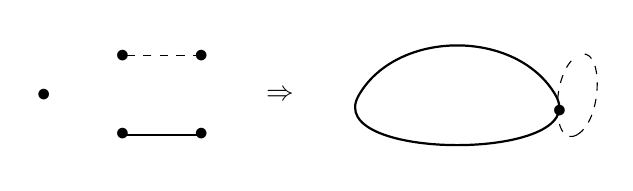
\begin{tikzpicture}
      \node () at (1,0) {$ \bullet $};
      \node () at (2,0.5) {$ \bullet $};
      \node () at (3,0.5) {$ \bullet $};
      \node () at (2,-0.5) {$ \bullet $};
      \node () at (3,-0.5) {$ \bullet $};
      \draw[dashed] (3,0.5) -- (2,0.5);
      \draw[thick] (3,-0.5) -- (2,-0.5);
      \node () at (4,0) { $ \Rightarrow $};
      \node () at (7.55,-0.2) {$ \bullet $};
      \draw[dashed] (7.775,-0.5) to[out=30, in=30] (7.775,0.5);
      \draw[dashed] (7.775,-0.5) to[out=210, in=-150] (7.775,0.5);
      \draw[thick] (7.5,0) to[out=120, in=60] (5,0);
      \draw[thick] (7.5,0) to[out=-60, in=-120] (5,0);
    \end{tikzpicture}
    \caption{Primo attaccamento per la costruzione del toro. Successivamente
      si attacca un disco deformato a forma di rettangolo identificando due lati
      opposti con la linea solida e gli altri due lati con la linea tratteggiata.
      Il risultato è, con un minimo di immaginazione, un toro.}
  \end{figure}
\end{example}

\begin{example}[Prodotto di sfere]
  Siano $ X = \Sph{p} $ e $ Y = \Sph{q} $, questi spazi sono formati
  da una $ 0 $-cella, e da un'altra cella di dimensione $ p $ o $ q $
  con mappe di attaccamento costanti. Anche lo spazio $ X \times Y $ può essere
  strutturato come CW complesso.
  % Sia $ X = \Sph{p} $ allora una possibile struttura di CW
  % è data da una $ 0 $-cella $ e_0 $ e una $ p $-cella $ e_p $.
  % Allora $ X^{(0)} = \set{X} $, $ X^{(p)} = \set{X} \cup_f \Disk{p} $
  % e $ f \colon \Disk{p} \to \Sph{p} $ con $ f \big \vert_{\partial \Disk{p}} = \mathrm{cost.} $.
  % $ Y = \Sph{q} $ con $ f_0 $ $ 0 $-cella, $ f_q $ $ q $-cella,
  % la mappa di attaccamento è: $ g \colon \Disk{q} \to \Sph{q} $ con $ g \big \vert_{\partial \Disk{p}} = \mathrm{cost.} $.
  Questo possiede una $ 0 $-cella $ e_0 \times f_0 $, una $ p $-cella
  $ e_p \times f_0 $, una $ q $-cella $ e_0 \times f_q $ e una $ (p + q) $-cella
  $ e_p \times f_q $. Lo $ 0 $-scheletro è formato da $ \set{(x,y)} $ con $ x \in \Sph{p} $ e $ y \in \Sph{q} $,
  e le mappe di attaccamento sono:

  \noindent
  Per la $ p $-cella:
  \begin{align*}
    F_{p0} \colon \Disk{p} & \to \Sph{p} \times \Sph{q} \\
    z & \mapsto (f(z), y)
  \end{align*}
  Per la $ q $-cella:
  \begin{align*}
    F_{0q} \colon \Disk{q} & \to \Sph{p} \times \Sph{q} \\
    z & \mapsto (z, g(u))
  \end{align*}
  Per la $ (p+q) $-cella:
  \begin{align*}
    F_{pq} \colon \Disk{p+q} & \to \Sph{p} \times \Sph{q} \\
    (w,u) & \mapsto (f(w), g(u))
  \end{align*}
  Dove $ f $ e $ g $ sono le mappe che realizzano gli attaccamenti in $ X $ e in $ Y $,
  cioè tali che sul bordo del disco siano costanti.
\end{example}
% \begin{example}
%   La sfera $ \Sph{n} $ per $ n \geq 0 $ possiede numerose strutture di CW complesso,
%   ad esempio una $ 0 $-cella e una $ n $-cella, oppure un politopo gonfiato.
% \end{example}

\section{Spazi proiettivi}

\subsection{Spazi proiettivi reali}


\newmathsymb{proreal}{\Pjr{n}}{Spazio proiettivo reale}
\begin{definition}
  Si definisce lo \textbf{spazio proiettivo reale}\index{Spazio proiettivo
    reale} come lo spazio quoziente $ \Pjr{n} = {\RN{n+1} \setminus \set{0}} \slash {\sim} $ con
  $ \vec{x} \sim \vec{y} $ se e solo se $ \vec{x} $ e $ \vec{y} $ sono multipli,
  cioè se esiste $ \lambda \in \RN{} \setminus \set{0} $ tale che $ \vec{x} = \lambda \vec{y} $.
  Gli elementi di $ \Pjr{n} $ si indicano con $ [x_0 : \dots : x_n] $.
\end{definition}
Fissato $ j \in \set{0, \dots, n} $ e definito
$ U_j = \set{[x_0 : \dots : x_n] \in \Pjr{n} | x_j \not = 0 } $ si definisce la mappa:
\begin{align*}
  \phi_j \colon U_j & \to \RN{n} \\
  [x_0 : \dots : x_n] & \mapsto \left(\frac{x_0}{x_j}, \dots, \frac{x_n}{x_j}\right)
\end{align*}
Si dimostra che $ \phi_j $ è un omeomorfismo. Queste mappe permettono di definire la
topologia dello spazio proiettivo: un sottoinsieme di $ U_i $ è aperto se lo è
in $ \RN{n} $ attraverso $ \phi_i $, e un insieme generico $ A $ è aperto se lo
sono tutte le intersezioni con gli insiemi $ U_i $. In questo modo $ \Pjr{n} $ è
una varietà topologica di dimensione $ n $.

\begin{lemma}
  Si dimostra che $ \Pjr{n} \cong {\Sph{n}} \slash {H} $ con $ H = \set{\Id{\Sph{n}}, a_{\Sph{n}}} $, dove
  $ a $ è la mappa antipodale, cioè $ x \sim y \iff x = y \vee x = - y $.
\end{lemma}
\begin{proof} \emph{Sketch of proof.}
  La mappa che realizza questo omeomorfismo è:
  \begin{align*}
    f \colon \Pjr{n} & \to \quot{\Sph{n}}{\sim}\\
    [\vec{x}]_{\Pjr{n}} & \mapsto \left[\frac{\vec{x}}{||\vec{x}||}\right]_\sim
  \end{align*}
  La dimostrazione che questa è un omeomorfismo è piuttosto laboriosa. Il motivo è
  comunque intuitivo: lo spazio proiettivo reale è formato dalle rette che passano
  per l'origine, le quali possono tutte essere identificate da un vettore di modulo
  1 su una semisfera.
\end{proof}
\eproof
Per i primi spazi proiettivi reali:
\begin{itemize}
\item
  $ \Pjr{1} \simeq \Sph{1} \slash \sim \; \simeq \Sph{1} \simeq \RN{} \cup {\infty} $. Questa è una
  $ 1 $-cella e una $ 0 $-cella.
\item $ \Pjr{2} = \Sph{2} \slash \sim $, cioè si identifica l'emisfero Sud con quello
  Nord. Si può quindi costruire questo spazio attaccando una $ 2 $-cella
  ad una $ \Sph{1} $ e quindi facendo l'identificazione di antipodalità.
  Ma $ \Sph{1} = \Pjr{1} $ quindi $ \Pjr{2} = \mathbb{P}^1(\RN{}) \cup_\phi \Disk{2} $
  Ho $ {\Sph{2}} \slash {\sim} $, l'emisfero sud della sfera si identifica con quello
  con:
  \begin{align*}
    \phi \colon \partial \Disk{2} = \Sph{1} & \to \Pjr{1} = \Sph{1} \\
    (x,y) & \mapsto (-x,-y)
  \end{align*}
  \vspace*{-18pt}
  \begin{figure}[htbp]
    \centering
    \begin{tikzpicture}
      \fill[gray!20] (0,0) circle (1);
      \draw (0,0) circle (1);
      \draw[-Latex] (0.1,1) -- (0.1001,1);
      \draw[-Latex] (-0.0999,-1) -- (-0.101,-1);
      \node () at (1,0) {-};
      \node () at (-1,0) {-};
    \end{tikzpicture}
    \caption{$ \Pjr{2} $, attacco al disco una circonferenza con la mappa $ f $,
      che quindi identifica i punti antipodali.}
    \label{fig:lez10:projective}
  \end{figure}
\item Attaccando un ulteriore cella $ \Disk{3} $ si costruisce lo spazio $ \Pjr{3} $.
  In questo modo $ \Pjr{3} = \Pjr{2} \cup_\phi \Disk{3} $ con:
  \[
    \phi \colon \partial \Disk{3} = \Sph{2} \to \Pjr{2} = \quot{\Sph{2}}{\sim}
  \]
  Si sceglie come mappa $ \phi $ la proiezione al quoziente su
  $ \Sph{2} \slash \sim $ in questo modo è automaticamente realizzata l'identificazione
  antipodale che definisce gli spazi proiettivi.
\end{itemize}
Continuando ad aggiungere una cella alla volta e scegliendo sempre
la mappa di proiezione al quoziente si ottengono tutti gli spazi proiettivi reali.
\begin{lemma}%[Struttura CW complessa degli spazi proiettivi reali]
  Sia $ X^{(k+1)} = \Pjr{k} \cup_\phi \Disk{k+1} $ con
  \[
    \phi \colon \partial \Disk{k+1} = \Sph{k} \to \Pjr{k} = \quot{\Sph{k}}{\sim}
  \]
  mappa di proiezione al quoziente, allora $ X^{(k+1)} \simeq \Pjr{k+1} $.
\end{lemma}
\begin{proof}
  Costruisco esplicitamente un omeomorfismo $ \Phi \colon X^{(k+1)} \to \mathbb{P}^{k+1}(\RN{}) $,
  per far ciò definisco una mappa $ \eta :  \mathbb{P}^{k}(\RN{}) \sqcup \Disk{k+1} \to \Pjr{\RN{}} $
  che si porta al quoziente:
  \[
    \begin{tikzcd}
      \mathbb{P}^{k}(\RN{}) \sqcup \Disk{k+1} \arrow{r}{\eta} \arrow{d}{P} &  \mathbb{P}^{k+1}(\RN{}) \\
      X^{(k+1)} \arrow{ru}{\Phi}
    \end{tikzcd}
  \]
  Una possibile costruzione di $ \eta $ è con le mappe
  \begin{align*}
    i \colon \mathbb{P}^{k}(\RN{}) & \to \mathbb{P}^{k+1}(\RN{})  \\
    [z_0 : \dots : z_k] & \mapsto [z_0: \dots: z_k: 0]
  \end{align*}
  E:
  \begin{align*}
    j \colon \Disk{k+1} & \to \mathbb{P}^{k+1}(\RN{}) \\
    (z_0, \dots, z_k) & \mapsto  \left[z_0: \dots: z_{k+1} = \sqrt{1 - \sum_{j=1}^k z_i^2}\right]
  \end{align*}
  Siccome $ \sum_{j=1}^k z_i^2 \leq 1 $ l'applicazione è ben definita, quindi $ \eta = (i,j) $.
  % \begin{exercise}
  %   Dimostrare che $ \eta $ è continua e gode di tutte le buone proprietà che le
  %   sono richieste.
  % \end{exercise}
  Rimane da dimostrare che $ \eta $ è continua e gode di tutte le buone proprietà che le
    sono richieste.
\end{proof}

  % Lo spazio proiettivo reale di dimensione $ n $ $ \Pjr{n} $ possiede una
  % struttura di CW complesso con una $ 0 $-cella, una $ 1 $-cella, \dots, una
  % $ n $-cella. Lo $ 0 $-scheletro è un punto, l'$ 1 $-scheletro è
  % $ K^{(1)} = K^{(0)} \cup_{f_0} \Disk{1} \cong \Pjr{1} $ che è una retta proiettiva
  % reale, il $ 2 $-scheletro è
  % $ K^{(2)} = K^{(1)} \cup_{f_1} \Disk{1} \cong \Pjr{2} $ che è un piano proiettivo
  % reale, e cosí via con $ f_j \colon \partial \Disk{j} \to K^{(j-1)} $ per
  % $ j \geq 1 $. In generale ho
  % $ \phi_j \colon \Disk{j} \to K^{(j-1)} \cong \Pjr{j-1} $. $ \Pjr{j-1} $ contiene
  % $ \Pjr(j-2) $ come iperpiano all'infinito, ad esempio $ z_{j-1} = 0 $. Poi a
  % $ \Pjr{j-2} $ incollo $ \Sph{j-2} $ tramite la mappa antipodale. Ad esempio
  % per $ n = 2 $ $ \Pjr{2} $ contiene
  % $ \Pjr{1} = \set{ [z_0 : z_1 : 0] | (z_0, z_1) \not = 0 } $. Attacco
  % $ \Disk{2} $ su questo $ \Pjr{1} $ con:
  % \begin{align*}
  %   f \colon \Sph{1} = \partial \Disk{2} & \to \Pjr{1} \\
  %   z & \mapsto [z]
  % \end{align*}
  % Che è la proiezione sul quoziente (mappa antipodale), infatti
  % $ \Pjr{1} = \quot{\Sph{1}}{H} $. %Quindi $ \Pjr{2} = \Pjr{1} \cup_f \Disk{2} $.


\subsection{Spazi proiettivi complessi}

\newmathsymb{pjc}{\Pjc{n}}{Spazio proiettivo complesso}
\newmathsymb{cstar}{\C^\star}{Piano complesso privato dell'origine}
\begin{definition}
Lo \textbf{spazio proiettivo complesso}\index{Spazio proiettivo complesso} è definito da :
\[
  \Pjc{n} = \quot{\C^{n+1} \setminus \set{\vec{0}}}{\sim}
\]
con la relazione:
\[
  (z_0, \dots, z_n) \sim (w_0, \dots, w_n) \iff \exists \lambda \in \C^\star= \C \setminus \set{0} \text{ tali che } z_i = \lambda w_i \; \forall i \in \set{0, \dots, n}
\]
\end{definition}
Questo è uno spazio compatto, connesso, di Hausdorff i cui punti si indicano con
$ p = [z_0 : \dots : z_n] $. Utilizzando la stessa costruzione dello spazio proiettivo
reale si rende $ \Pjc{n} $ una varietà topologica di dimensione reale $ 2n $.
\begin{lemma}
  Equivalentemente si ha che lo spazio proiettivo complesso è:
  \[
    \Pjc{n} \simeq \quot{\Sph{2n+1}}{{\sim}}
  \]
  Dove $ z \sim w $ se $ z $ e $ w $ sono numeri complessi che differiscono per al
  più una fase, cioè se $ \exists \lambda \in \mathbb{C} $ con
  $ | \lambda | = 1 $ tale che $ z = \lambda w $. Equivalentemente si può dire che
  $ \sim $ è l'azione di $ \Sph{1} $ su $ \Sph{2n+1} $ e quindi si può vedere
  $ \Pjc{n} $ come le orbite di $ \Sph{2n+1} $ sotto l'azione di $ \Sph{1} $.
\end{lemma}
\begin{proof}
  L'isomorfismo è realizzato da:
  \begin{align*}
    \Pjc{n} = \quot{\mathbb{C}^{n+1}}{\sim} & \to  \quot{\Sph{2n+1}}{\sim} \\
    [z]_{\Pjc{n}} & \mapsto \left[\frac{x}{|| x ||}\right]_\sim
  \end{align*}
  Come si può verificare con tediosi calcoli.
\end{proof}
\begin{osservation}
  Si osserva che $ \Pjr{n} $ è lo spazio dei possibili sottospazi di dimensione
  $ 1 $ in $ \RN{n+1} $ mentre $ \Pjc{n} $ è lo spazio dei possibili sottospazi
  di dimensione $ 1 $ in $ \mathbb{C}^{n+1} $.
\end{osservation}
% Fissato $ j \in \set{0, \dots, n} $ e definito
% $ U_j = \set{[z_0, \dots, z_n] \in \Pjc{n} | z_j \not = 0 } $ si definisce la mappa:
% \begin{align*}
%   \phi_j \colon U_j & \to \C^n \simeq \RN{2n} \\
%   [z_0, \dots, z_n] & \mapsto \left(\frac{z_0}{z_j}, \dots, \frac{z_n}{z_j}\right)
% \end{align*}
% Si dimostra che $ \phi_j $ è omeomorfismo. Queste mappe permettono di definire la
% topologia dello spazio proiettivo: un sottoinsieme di $ U_i $ è aperto se lo è
% in $ \RN{2n} $ attraverso $ \phi_i $, e un insieme generico $ A $ è aperto se lo
% sono tutte le intersezioni con gli insiemi $ U_i $. In questo modo $ \Pjc{n} $ è
% una varietà topologica di dimensione $ 2n $.
\begin{example}[$ n = 1 $]
  $ \Pjc{1} $ è noto come retta complessa o sfera di Riemann, in quanto
  si trova che $ \Pjc{1} \simeq \Sph{2} $, infatti usando le mappe di isomorfismo $ \phi_i $:
  \[
    \Pjc{1} = \set{ [0:1] } \cup U =: \set{\infty} \cup U
  \]
  Con $ U $ intorno aperto omeomorfo a $ \RN{2} $. Ma la proiezione
  stereografica manda la sfera senza polo Nord in $ \RN{2} $, cioè
  $ \Sph{2} \setminus \set{N} \simeq \RN{2} $, quindi
  $ \Pjc{1} \setminus \set{\infty} \simeq \RN{2} $ e quindi
  $ \Pjc{1} \setminus \set{\infty} \simeq \Sph{2} \setminus \set{N} $. Questi sono spazi non compatti ma
  di Hausdorff, so che la compattificazione di Alexandroff\footnotemark sono
  spazi omeomorfi, ma la compattificazione di uno spazio meno un punto è lo
  spazio stesso: $ \Pjc{1} \simeq \Sph{2} $. Questo spazio ammette una costruzione di
  CW complesso. $ K^{(0)} $ è un punto $ \Pjc{0} $, poi si può costruire
  $ K^{(2)} = K^{(0)} \cup_f \Disk{2} = \Sph{2} \simeq \Pjc{1} $ con $ f $ mappa
  costante, che quindi fa collassare il bordo in un punto. Successivamente si ha
  $ K^{(4)} = K^{(2)} \cup_\pi \Disk{4} $ infatti $ K^{(2)} = \Pjc{1} $, poi prendo
  $ \Disk{4} $ so che $ \partial \Disk{4} = \Sph{3} $ e la mappa al quoziente è
  $ \pi \colon \Sph{3} \to \Pjc{1} $ che è fatta così:
  \begin{align*}
    \pi \colon \Sph{3} & \mapsto \Pjc{1} \\
    (z_0, z_1) & \mapsto [z_0 : z_1]
  \end{align*}
  Posso fare agire $ \Sph{1} $:
  \begin{align*}
    \Sph{1} \times \Sph{3} & \to \Sph{3} \\
    (\lambda, (z_0, z_1)) & \mapsto (\lambda z_0, \lambda z_1)
  \end{align*}
  Siccome $ \lambda \in \Sph{1} $ allora $ | \lambda | = 1 $ e quindi $ | \lambda z_0 |^2 + | \lambda z_1 |^2 = 1 $.
  Faccio il quoziente $ \Pjc{1} = \quot{\Sph{3}}{\Sph{1}} $ e $ \pi $ è la proiezione al
  quoziente.
\end{example}
\footnotetext{\index{Compattificazione di Alexandroff}La compattificazione di
  Alexandroff consiste nell'aggiungere un punto ad uno spazio topologico per
  renderlo compatto.}

% In merito al generico spazio proiettivo complesso $ \Pjc{n} $ vorrei sapere
% quale è la struttura di CW complesso, quale è il suo gruppo fondamentale e quali
% sono i suoi gruppi di omologia.

In generale $ K^{(2n - 2)} $ si costruisce prendendo $ \Disk{2n} $ e con la mappa
di proiezione $ \pi \colon \partial \Disk{2n} = \Sph{n-1} \to \Pjc{n-1} $, quindi $ K^{(2n -2)} \cup_\pi \Disk{2n} $.
$ \Pjc{n} $ è un CW complesso ottenuto attaccando celle di dimensione $ 2j $ per $ 0 \leq j \leq n $
Quindi ho una $ 0 $-cella, una $ 2 $-cella, \dots, una $ 2n $-cella.

\begin{osservation}
  In generale $ \Pjc{n} = \Pjc{n-1} \cup \C^n $. Procedendo induttivamente:
  $ \Pjc{n} = \Pjc{n-1} \cup \C^n = \Pjc{n-2} \cup \C^{n-1} \cup \C^{n} = \dots $.
\end{osservation}

\begin{proposition}
  Vale che $ K^{(2n)} \simeq \Pjc{n} $.
\end{proposition}
\begin{proof}
  La dimostrazione è per induzione. Per $ t = 1 $ l'ho già verificato, assumo
  che $ K^{(2t)} = \Pjc{t} $ per $ 0 \leq t \leq n-1 $.

  Sia
  \begin{align*}
    h \colon \Disk{2n} & \to \Pjc{n} \\
    (z_0, \dots, z_{n-1}) & \mapsto \left[z_0:\dots: z_{n-1}:\sqrt{1 - \sum_{i < n}|z_i|^2} \right]
  \end{align*}
  So che $ \partial \Disk{2n} = \Sph{2n-1} = \set{|z_0|^2 + \dots + |z_{n-1}|^2 = 1} $
  quindi $ h $ è ben definita in quanto la radice esiste, ed è continua.
  Restringendo $ h $ su $ \partial \Disk{2n} $ si ha che $ \sum_{i < n}|z_i|^2 = 1 $,
  quindi:
  \begin{align*}
    h \big \lvert_{\partial \Disk{2n}} \colon \Sph{2n-1} & \to \Pjc{n-1} \\
    (z_0, \dots, z_{n}) & \mapsto [z_0: \dots: z_{n-1}: 0]
  \end{align*}
  Ma se $ P $ è un punto in $ \Pjc{n-1} $ allora:
  \[
    \left( h \big \lvert_{\partial \Disk{2n}}\right)^{-1}(P) = \set{ (\lambda_{z_0}, \dots, \lambda_{z_{n-1}}) | |\lambda| = 1, \sum|z_i|^2 = 1} %\simeq \Sph{1}
  \]
  Quindi $ h $ non è iniettiva (infatti tutti si possono scalare tutte le
  coordinate nello spazio proiettivo di un medesimo fattore e si ottiene sempre
  lo stesso punto). Quindi:
  \[
    \begin{tikzcd}
      \Pjc{k-1} \sqcup \Disk{2n} \rar{h} \dar{P} & \Pjc{n} \\
      \Pjc{n-1} \cup_\tau \Disk{2n} \arrow{ur}{F} & {}
    \end{tikzcd}
  \]
  Dove $ \tau $ realizza la proiezione al quoziente
  $ \tau \colon \Sph{2k-1} \to \Pjc{k-1} = \Sph{2k-1} \slash \Sph{1} $, mentre
  $ P $ è tale che $ P((z_0, \dots, z_{n-1})) = ([z_0, \dots, z_{n-1}]) $. $ F $ manda
  $ \Pjc{n-1} $ in $ \Pjc{n} $ banalmente e raccorda bene i dischi in quanto i
  punti che sono al quoziente finiscono tutti nel medesimo punto, giacché sono i
  punti tali che $ \sum | z_i |^2 = 1 $. $ F $ è iniettiva e suriettiva da uno
  spazio compatto a uno spazio di Hausdorff, quindi è un omeomorfismo.
\end{proof}
\eproof
Ho che $ \pi_1(\Pjc{n}) = \set{1} $ $ \forall n \geq 1 $
infatti per $ n = 1 $ $ \pi_1(\Pjc{1}) \cong \pi_1(\Sph[1]) = \set{1} $.
Per induzione suppongo che $ \pi_1(\Pjc{n-1}) = \set{1} $, voglio
mostrare che $ \pi_1(\Pjc{n}) = \set{1} $. Per fa ciò
uso il teorema di Seifert-van Kampen.
\[
  \Pjc{n} = \Pjc{n-1} \cup_\pi \Disk{2n}
\]
Considero $ x \in \Disk{2n} $ e un aperto $ V $ disco centrato in $ x $
di raggio $ \epsilon $ piccolo, cioè $ V = \Disk{2n}_\epsilon(x) $. Poi prendo
$ U = \Pjc{n} \setminus \set{x} $ aperto.
Vale che $ V \sim \set{x} $, poi $ \Disk{2n} $ si ritrae al bordo, che
si attacca. $ U \simeq \Pjc{n-1} $.
Poi $ V \cap U $ è una specie di corona circolare in $ \Disk{2n} $,
quindi $ V \cap U \sim \Sph{2n -1} $. Quindi $ \pi_1(\Pjc{n}) = \Pjc{n-1} \cong \set{1} $.
È più interessante vedere l'omologia singolare.
Si trova che:
\[
  H_k(\Pjc{n}) \cong
  \begin{cases}
    \Z & \text{se } k \in \set{0,2,4,\dots, 2n} \\
    0 & \text{altrimenti}
  \end{cases}
\]
Con $ k = 1 $ è il gruppo fondamentale, quindi è nullo, e poi torna per $ n = 1 $.

% Per comodità si introduce l'omologia cellulare di $ X $.

% Se $ X $ è spazio topologico con struttura di CW complesso si introduce
% l'omologia cellulare $ H_k^{CW}(X) $.

% Si trova che $ H_k^{CW}(X) \cong H_k(X) $ e c'è un algoritmo per calcolare $ H_k^{CW}(X) $.

% So che $ \Pjc{n} = \Pjc{n-1} \cup_\pi \Disk{2n} $. Fisso $ n $ voglio calcolare
% $ H_s(\Pjc{n}^{(t)}, \Pjc{n}^{(t-1)}) $.
% Calcolo per induzione.
% So che $ H_k(\Pjc{1}) $ è a posto, voglio calcolare $ H_k(\Sph{m}) $ per induzione.

% Mi piacerebbe che:
% \[
%   H_s(\Pjc{c}^{(t)}, \Pjc{n}^{(t-1)}) \cong H_s(\quot{\Pjc{n}^{(t)}}{\Pjc{n}^{(t-1)}})
% \]

% Questo è vero in generale, se $ A \subseteq X $ CW complessi allora:
% \[
%   H_k(X,A) \cong H_k(\quot{X}{A})
% \]
% Ma $ \Pjc{n}^{(t)} = \Pjc{n}^{(t-1)} \cup_\pi \Disk{2t} $, è come se collassa
% quello che è in comune alle celle, cioè il bordo del dei dischi ad un punto,
% cioè:
% \[
%   \quot{\Pjc{n}^{(t)}}{\Pjc{n}^{(t-1)}} \simeq \Sph{2t}
% \]
% Se $ s \not = 2 t $ allora $ H_s(\quot{\Pjc{n}^{(t)}}{\Pjc{n}^{(t-1)}}) = 0 $.
% \[
%   H_{2t}(\Pjc{n}^{(t)}, \Pjc{n}^{(t-1)}) \cong \Z
% \]
% E gli altri sono zero.

% In generale $ X^{(k)}- X^{(k-1)} \cup_{f_1} \Disk{k}_{\alpha_1} \cup \dots \cup_{f_n} \Disk{k}_{\alpha_N} $
% cosa è $ H_s(X^{(k)}, X^{(k-1)}) $.
% \[
%   H_s(X^{(k)}, X^{(k-1)}) \cong H_s(\quot{X^{(k)}}{X^{(k-1)}})
% \]
% Ma $ \quot{X^{(k)}}{X^{(k-1)}} $ è un bouquet, in quanto tutte le sfere hanno in comune
% il punto a cui si è contratto $ X^{(k-1)} $.
% Quindi:
% \[
%   H_s(X^{(k)}, X^{(k-1)}) \cong
%   \begin{cases}
%     \Z^N & \text{se } k = s \\
%     0 & \text{se } k \not = s
%   \end{cases}
% \]

% Considero $ \Pjc{n} $ ho che:
% \[
%   \Pjc{n-2} \incl \Pjc{n-1} \incl \Pjc{n}
% \]
% Quindi:
% \[
%   (\Pjc{n-1}, \Pjc{n-2}) \to (\Pjc{n}, \Pjc{n-1})
% \]
% e quindi
% \[
%   H_s(\Pjc{n-1}, \Pjc{n-2}) \to H_s(\Pjc{n}, \Pjc{n-1})
% \]
% Ma il primo è diverso da zero se $ s = 2n - 2 $ e
% il secondo è diverso da zero se $ s = 2n $.

% Da qui non ottengo informazioni di carattere generale,
% cioè quello che sto dicendo è che non è semplicemente
% la composizione della coppia allora uso un trucco.

% Costruisco un'applicazione. FORSE

% % Sia $ X $ un CW complesso e $ Y $ un CW complesso, è
% % possibile dare una struttura di CW complesso anche a $ Z = X \times Y  $.
% % Se $ \set{e_\alpha} $ sono le celle di $ X $ e $ \set{f_\beta} $
% % quelle di $ Y $, allora $ \set{e_\alpha \times f_\beta} $ sono
% % celle di $ Z $. Bisogna solo capire come sono fatte le
% % mappe di attaccamento.

    %     lezione 8

\section{(ex-)Congettura di Poincaré}

Per $ n = 2 $ ho $ \Sph{2} $ è una $ 2 $-varietà topologica compatta e connessa
il cui gruppo fondamentale è banale e i gruppi di omologia noti, infatti ho
calcolato l'omologia di una sfera generica:
\[
  H_k(\Sph{n}) \cong
  \begin{cases}
    \Z & \text{ se } k \in \set{0,n} \\
    0 & \text{ se } k \not \in \set{0,n}
  \end{cases}
\]
In particolare ho $ H_0(\Sph{n}) \cong \Z $ ed è generato dalla classe di
omologia di un punto qualsiasi, mentre $ H_n(\Sph{n}) \cong \Z $ è generato dalla
classe di omologia di un $ n $-simplesso singolare $ \tau_n \colon \Delta_n \to \Sph{n} $.

\begin{proposition}
  Se $ \M $ è una $ 2 $-varietà topologica compatta e connessa tale che $ \forall k \leq 2 $
  $ H_k(\M) \cong H_k(\Sph{2}) $ allora $ \M \simeq \Sph{2} $.
\end{proposition}
\begin{proof}
  Esiste un teorema di classificazione delle varietà topologiche di dimensione
  $ 2 $ compatte e connesse, questo dice che una varietà topologia $ \M $
  compatta e connessa di dimensione $ 2 $ è omeomorfa a una delle seguenti tre
  categorie: $ \Sph{2} \simeq V_0 $, $ V_g $ oppure $ U_n $. Dove:
  \[
    V_g =
    \begin{cases}
      \Sph{2} & \text{se } g = 0 \\
      \quot{P_{4g}}{\sim} & \text{se } g \geq 1
    \end{cases}
  \]
  Dove $ \sim $ è l'identificazione $ a_1 b_1 a_1^{-1}b_1^{-1}\dots a_g b_g a_g^{-1}b_g^{-1} $,
  come ad esempio il toro, mentre:
  \[
    U_n =
    \begin{cases}
      \mathbb{P}^2(\RN{}) & \text{se } n = 1 \\
      \quot{P_{2n}}{\sim} & \text{se } n \geq 2
    \end{cases}
  \]
  Con $ \sim $ è l'identificazione $ a_1 a_1 \dots a_n a_n $, come ad esempio la
  bottiglia di Klein ($ abab^{-1} = aabb $). Tutti i $ V_g $ non sono omeomorfi
  tra loro, e similmente gli $ U_n $, e neppure gli $ U_n $ e i $ V_g $ sono
  vicendevolmente omeomorfi in quanto i primi sono non orientabili, mentre i
  secondi si. Escludo queste due possibilità confrontando i primi gruppi di
  omologia. So che:
  \[
    H_1(V_g) \cong
    \begin{cases}
      H_1(\Sph{2}) & \text{se } g = 0 \\
      \Z^{2g} & \text{se } g \geq 1
    \end{cases}
  \]
  Gli spazi $ V_g $ con $ g \geq 1 $ non hanno lo stesso tipo di omologia di
  $ \Sph{2} $ perché $ H_1(V_g) $ è non banale, mentre il gruppo fondamentale di
  $ \Sph{2} $ lo è. Similmente
  $ H_1(\mathbb{P}^2(\RN{})) \cong \pi_1(\mathbb{P}^2(\RN{})) \cong \Z_2 $, che non è
  banale, e $ H_1(U_n) \cong \Ab{\pi_1(U_n)} $, ma usando Seifert-van Kampen si trova che:
  \begin{gather*}
    \pi_1(U_n) = \langle a_1, \dots, a_n \; | \; a_1^2\dots a_n^2 = 1 \rangle \; \Rightarrow \\
    \Ab{\pi_1(U_n)} = \langle a_1, \dots, a_n \; | \;  c = a_1 \dots a_n = \pm 1 \rangle = \Z_2 \oplus \Z^{n-1}
  \end{gather*}
  Dove $ \Z_2 $ viene dal fatto che abelianizzando si ha
  $ c = a_1^2\dots a_n^2 = (a_1 \dots a_n)^2 = 1 $ quindi $ c = \pm 1 $, mentre
  $ \Z^{n-1} $ è il gruppo libero generato dai rimanenti. Questo non è banale,
  quindi l'unico spazio possibile è proprio $ \Sph{2} $.
\end{proof}
\eproof
Per $ \Sph{3} $ vale il seguente risultato, dimostrato da Perelman nel
2003, precedentemente noto come congettura di Poincaré:
\begin{proposition}[ex-Congettura di Poincaré]
  Se $ \M $ è una $ 3 $-varietà topologica compatta, connessa e semplicemente
  connessa tale che $ \forall k \leq 3 $ $ H_k(\M) \cong H_k(\Sph{3}) $ allora $ \M \simeq \Sph{3} $.
\end{proposition}
Se rinuncio alla richiesta di semplice connessione il risultato non vale più, ma
vale la seguente proposizione:
\begin{proposition}
  Se $ \M $ è una $ 3 $-varietà topologica compatta e connessa tale che $ \forall k \geq 3 $
  $ H_k(\M) \cong H_k(\Sph{3}) $ allora non si può concludere che $ \M \simeq \Sph{3} $.
\end{proposition}
\newmathsymb{mat}{M_n(\mathbb{F})}{Matrici quadrate di ordine $ n $ sul campo $ \mathbb{F} $}
\begin{proof}
  Costruisco un controesempio, noto come \textbf{spazio dodecaedrico di
    Poincaré}\index{Spazio dodecaedrico}, o anche spazio a omologia
  razionale\index{Spazio a omologia razionale ! \vedi{Spazio dodecaedrico}}.
  Costruirò una $ 3 $-varietà topologica compatta e connessa $ P $ con lo stesso
  tipo di omologia di una $ 3 $-sfera ma non omeomorfa a $ \Sph{3} $ in quanto
  il gruppo fondamentale è finito non abeliano di ordine 120. Parto da
  $ \Sph{3} $, posso scrivere:
  \[
    \Sph{3} \subseteq \mathbb{C}^2 \qquad \Sph{3} = \set{ (z_0, z_1) \in \mathbb{C}^2 | |z_0|^2 + |z_1|^2 = 1}
  \]
  Infatti $ z_0 = x + i y $ e $ z_1 = t + i w $ quindi $ |z_0|^2 = (x + iy)(x - iy) = x^2 + y^2 $
  e $ |z_0|^2 = (t + iw)(t - iw) = t^2 + w^2 $ e quindi ottengo:
  \[
    \Sph{3} = \set{ (x,y,t,w) \in \RN{4} | x^2 + y^2 + t^2 + w^2 = 1}
  \]
  Così come $ \Sph{1} $ ha una struttura di gruppo U(1) è possibile strutturare
  $ \Sph{3} $ come gruppo SU(2):
  \[
    \mathrm{SU(2)} = \set{A \in M_2(\mathbb{C}) | \det{A} = 1, \; AA^\dagger = \Id{2}}
  \]
  Quindi $ \mathrm{SU(2)} \subseteq \mathbb{C}^4 $, si dimostra che $ A \in \mathrm{SU(2)} $ se e solo se
  è della forma:
  \[
    \begin{pmatrix}
      \alpha & - \beta^\star \\
      \beta & \alpha^\star \\
    \end{pmatrix}
    \text{ con } \alpha,\beta \in \mathbb{C} \text{ e } |\alpha|^2 + |\beta|^2 = 1
  \]
  % Questo significa che i vettori in $ \mathbb{C}^2 $ $ (\alpha, \beta) $ e
  % $ (-\beta^\star, \alpha^\star) $ sono normalizzati e sono tra di loro ortogonali.
  In questo modo si costruisce immediatamente la corrispondenza buinivoca tra
  SU(2) e $ \Sph{3} $:
  \begin{align*}
    \mathrm{SU(2)} & \leftrightarrow \Sph{3} \\
    \begin{pmatrix}
      \alpha & - \beta^\star \\
      \beta & \alpha^\star \\
    \end{pmatrix} & \leftrightarrow (\alpha,\beta)
  \end{align*}
  In questo modo si può definire un prodotto su $ \Sph{3} $ rappresentando
  $ (x,y,t,w) \in \RN{4} $ come numeri complessi e passando alla controparte
  matriciale, dove il prodotto è definito naturalmente come prodotto riga per
  colonna, quindi una volta svolto il prodotto si torna alla notazione a quattro
  reali. A questo punto è triviale trovare l'identità e l'elemento inverso che
  permettono di dare a $ \Sph{3} $ la struttura di gruppo. Inoltre vedendo SU(2)
  come spazio topologico con topologia indotta da $ \mathbb{C}^4 $ SU(2) e
  $ \Sph{3} $ sono sia isomorfi come gruppi che omeomorfi come spazi topologici.

  La costruzione dello spazio dodecaedrico si basa sulle isometrie del dodecaedro $ D_{12} $,
  questo è un solido regolare con 12 facce, 30 spigoli e 20 vertici.
  \begin{figure*}[htbp]
    \centering
    \def\svgwidth{0.26\textwidth}
    \input{images/Dodecahedron.pdf_tex}
    \caption{Dodecaedro}
  \end{figure*}

  \noindent
  Il gruppo di isometrie del dodecaedro, cioè:
  \[
    \mathrm{Isom}(D_{12}) = \set{ g \colon \RN{3} \to \RN{3} | g \text{ regolare e } g(D_{12}) = D_{12}}
  \]
  Questo gruppo si può vedere come:
  \[
    \mathrm{Isom}(D_{12}) \cong A_5 \times \Z_2
  \]
  Dove $ A_5 $ è un sottogruppo di $ \mathrm{Isom}(D_{12}) $ ed è il gruppo
  alterno (cioè il gruppo delle permutazioni pari) su 5 elementi e quindi ha ordine 60.
  Le 60 trasformazioni che sono in $ A_5 $ sono l'identità, 24 rotazioni di $ \frac{2}{5} \pi $ attorno
  agli assi per i centri di facce opposti, 20 rotazioni di $ \frac{2}{3} \pi $ attorno
  agli assi per vertici opposti e 15 rotazioni di $ \pi $ attorno agli assi per
  i punti medi di spigoli opposti.
  $ \Z_2 $ invece è dovuto all'applicazione antipodale che è $ (x,y,z) \mapsto (z,y,z) $.
  $ A_5 $ è un sottogruppo finito di SO(3) che sono le rotazioni di $ \RN{3} $ attorno
  a una retta passante per l'origine, cioè:
  \[
    \mathrm{SO(3)} = \set{ R \in M_3(\RN{}) | \det{R} = 1, \;R^T R = \Id{3}}
  \]
  Per passare da SO(3) a $ \Sph{3} $ utilizzo la \textbf{rappresentazione spinoriale}\index{Rappresentazione spinoriale di SO(3)}
  (questo mi permette di passare dal dodecaedro che è tridimensionale alla $ 3 $-sfera).
  Sia $ \rho $ una rappresentazione di SU(2), cioè un omomorfismo:
  \[
    \rho \colon \Sph{3} = \mathrm{SU(2)} \to \mathrm{GL}(V)
  \]
  Con GL gruppo generale lineare e $ V $ è uno spazio vettoriale di dimensione
  3 (quindi $ V \simeq \RN{3} $) che scelgo essere lo spazio delle matrici antihermitiane a
  traccia nulla:
  \[
    V = \set{H \in M_2(\mathbb{C}) | H + H^\dagger = 0, \; \tr H  = 0}
  \]
  Si trova che $ V $ è generato da:
  \[
    E_1 =
    \begin{pmatrix}
      0 & i \\
      i & 0 \\
    \end{pmatrix}
    \quad
    E_2 =
    \begin{pmatrix}
      0 & 1 \\
      -1 & 0 \\
    \end{pmatrix}
    \quad
    E_3 =
    \begin{pmatrix}
      i & 0 \\
      0 & -i \\
    \end{pmatrix}
  \]
  Allora scelgo $ \rho(T) \colon H \mapsto THT^\dagger $.
  Perché $ \rho $ sia una rappresentazione bisogna verificare che se $ T \in \mathrm{SU(2)} $
  e $ H \in V $:
  \begin{enumerate}
  \item $ \rho $ omomorfismo
  \item $ \rho(T) $ lineare
  \item $ \rho(T) $ invertibile
  \item $ \rho(T)(H) \in V $
  \end{enumerate}
  Verifico ad esempio che $ \rho(T)(H) \in V $:
  \begin{gather*}
    THT^\dagger + TH^\dagger T^\dagger = 0 \iff T(H + H^\dagger)T^\dagger = 0 \iff H \in V \\
    \tr(THT^\dagger) = \tr(THT^{-1}) \overset{\text{ciclicità}}{=} \tr(H) = 0 \iff H \in V
  \end{gather*}
  Ho quindi $ \rho \colon \Sph{3} \to \mathrm{GL}(V) $, vorrei cercare di restringere a
  O($ V $) al posto di $ \mathrm{GL}(V) $. Per far ciò bisogna prima definire un
  prodotto scalare definito positivo, in modo da poter definire il concetto di
  isometria e considerare quindi O($ V $) come il gruppo di isometrie di $ \RN{3} $.
  Una possibile forma quadratrica naturale è in questo caso il determinante,
  infatti se $ H \in V $ allora:
  \[
    H =
    \begin{pmatrix}
      i a & c + i b \\
      -c + i b & - i a
    \end{pmatrix}
  \]
  Con $ a,b,c \in \RN{} $, infatti $ \det{H} = a^2 + b^2 + c^2 $ che è il consueto
  prodotto scalare in $ \RN{3} $. In questo modo $ V $ diventa uno spazio euclideo
  con prodotto scalare $ q = \det $.

  Con questa definizione $ \rho(T) \colon V \to V $ è un'isometria. Questo è vero se
  $ q(\rho(T)(H)) = q(H) $ cioè se $ \det(THT^\dagger) = \det{H} $, ma per Binet questo
  equivale a $ \det{T}\det{H}\det{T^\dagger} = \det{H} $, utilizzando il fatto che il
  determinante di una matrice è un numero complesso e quindi commuta questo
  equivale a $ \det{T}\det{T^\dagger}\det{H} = \det{H} $, sempre per Binet
  $ \det(TT^\dagger)\det{H} = \det{H} $, ma per ipotesi $ TT^\dagger = \Id{} $ quindi
  effettivamente $ \rho(T) $ è isometria, perciò:
  \[
    \rho \colon \Sph{3} \to \mathrm{O}_3(V) \; \text{cioè } \rho(T) \in \mathrm{O}_3(V)
  \]
  \vspace*{-20pt}
  \begin{exercise}
    Verificare che $ \rho $ è continua come applicazione tra spazi topologici
    equipaggiando $ \mathrm{O}_3(V) $ con la topologia indotta da $ \RN{9} $.
  \end{exercise}
  Essendo $ \rho $ continua manda compatti in compatti e connessi in connessi,
  quindi $ \rho(\Sph{3}= \mathrm{SU(2)}) $ è connesso in $ \mathrm{O}_3(V) $. Ma
  $ \mathrm{O}_3(V) $ non è connesso, e anzi è formato da due componenti
  connesse, una è SO(3), l'altra è SO(3) moltiplicata per una qualunque matrice
  di determinante $ - 1 $. Siccome $ \rho $ è omomorfismo
  $ \rho(\Id{}) = \Id{} $, quindi $ \rho(\Sph{3}) = \mathrm{SO(3)} $, in questo modo
  rappresento la $ 3 $-sfera come rotazioni in $ \RN{3} $. Si dimostra che
  $ \rho $ è suriettiva e $ \ker{\rho} = \set{(1,0,0,0), (-1,0,0,0)} $ elementi che
  corrispondono a $ \Id{} $ e $ -\Id{} $. A livello di gruppi per il primo
  teorema di omomorfismo:
  \[
    \quot{\Sph{3}}{\ker{\rho}} \cong \mathrm{SO(3)}
  \]
  Ad una rotazione in $ \RN{3} $ corrispondono due punti sulla $ 3 $-sfera che sono
  uno l'antipodale dell'altro.

  Ora ho $ A_5 \subseteq \mathrm{SO(3)} $ definisco
  $ G = \set{ T \in \Sph{3} | \rho(T) \in A_5} $, cioè sono tutti i punti della sfera a
  cui corrispondono le rotazioni in $ A_5 $. $ G $ è un gruppo, infatti se
  $ T, S \in G $ allora $ \rho(T), \rho(S) \in A_5 $ e
  $ \rho(TS) = \rho(T)\rho(S) \in A_5 $ in quanto $ A_5 $ gruppo e $ \rho $ omomorfismo.
  Inoltre $ \Id{} \in G $ in quanto $ \rho(\Id{}) \in A_5 $. Si definisce
  $ \phi = \rho \lvert_G \colon G \to A $, la quale per costruzione è suriettiva. Inoltre
  $ \ker{\phi} = \set{ T \in G | \phi(T) = \Id{}} $, ma $ \phi(T) = \rho(T) $, quindi
  $ T = \pm \Id{} $, cioè $ \ker{\phi} = \ker{\rho} = \set{- \Id{}, + \Id{}} $. Si può
  costruire la successione esatta di gruppi:
  \[
    \begin{tikzcd}
      \Id{} \arrow{r}{} & \ker{\phi} \arrow{r}{} & G \arrow{r}{} & A_5 \arrow{r}{} & \Id{}
    \end{tikzcd}
  \]
  Essendo la successione esatta vale che $ A_5 = {G} \slash {\ker{\phi}} $.
  $ G \subseteq \Sph{3} $ e ha ordine 120, inoltre $ \ker{\phi} $ è normale in
  $ G $. Si verifica formalmente che la successione spezza, quindi
  $ G \cong A_5 \oplus \ker{\phi} \cong \mathrm{Isom}(D_{12}) $, questo lo si intuisce per il
  fatto che sostanzialmente $ G $ e formato da $ (A_5, + \Id{}) $ e
  $ (A_5, - \Id{}) $. Ho quindi rappresentato $ A_5 $ in $ \Sph{3} $.
  Definendo l'azione del gruppo su $ \Sph{3} $:
  \begin{align*}
    G \times \Sph{3} & \to \Sph{3} \\
    (g,x) & \to gx
  \end{align*}
  Il prodotto $ gx $ va inteso in questo modo: sia $ g $ che $ x $ sono punti di
  $ \Sph{3} $, quindi sono rappresentabili come matrici di SU(2) per cui è ben
  definito il prodotto. Considerando la proiezione sul quoziente
  $ \pi \colon \Sph{3} \to {\Sph{3}} \slash {G} $ si definisce lo spazio dodecaedrico
  $ P := {\Sph{3}} \slash {G} $, il quale è connesso e compatto in quanto quoziente
  di uno spazio connesso e compatto. Lo spazio dodecaedrico è quindi la sfera
  con identificati tutti i punti che sono trasformabili l'uno nell'altro tramite
  l'azione di $ G $, che è il gruppo delle simmetrie del dodecaedro rappresentato
  sulla $ 3 $-sfera.
  Bisogna verificare:
  \begin{enumerate}
  \item $ P $ è una $ 3 $-varietà
  \item $ \pi_1(P) $ non è banale
  \item $ H_k(P) \cong H_k(\Sph{3}) \; \forall k \leq 3$
  \end{enumerate}
  Si dimostra che $ \pi $ è un rivestimento, cioè comunque si prenda un punto $ p \in P $
  esiste intorno di $ p $ a cui corrispondono 120 intorni disgiunti su $ \Sph{3} $.
  Siccome $ \Sph{3} $ è semplicemente connesso il rivestimento è universale.
  \begin{exercise}
    Dimostrare che $ \pi $ è rivestimento universale di $ P $ su $ \Sph{3} $.
  \end{exercise}
  Siccome $ P $ è rivestito da $ \Sph{3} $ è di dimensione 3 perché localmente è
  fatto come $ \Sph{3} $ che è una varietà $ 3 $-dimensionale. Dalla teoria
  generale dei rivestimenti si trova che $ \pi_1(P) \cong G $, quindi
  $ \pi_1(P) $ è non banale. Inoltre, $ P $ è connesso per archi perché passaggio
  al quoziente di insieme connesso per archi quindi $ H_0(P) \cong \Z $ cioè
  $ H_0(P) \cong H_0(\Sph{3}) $. Rimangono da calcolare i gruppi di omologia per
  $ k = 1 $ e $ k = 2 $, per far ciò considero $ \sigma \colon \Delta_k \to P $ un simplesso
  singolare, si ha il diagramma:
  \[
    \begin{tikzcd}
      {} & \Sph{3} \dar{\pi} \\
      \Delta_k \rar{\sigma} \arrow{ru}{} & P
    \end{tikzcd}
  \]
  Per il teorema di sollevamento $ \sigma \colon \Delta_k \to P $ induce una mappa
  $ \sigma' \colon \Delta_k \to \Sph{3} $. Se $ \sigma $ dà origine a un elemento non banale in
  $ H_k(P) $ anche $ \sigma' $ lo fa in $ H_k(\Sph{3}) $, ma per $ k \in \set{1,2} $
  $ H_k(\Sph{3}) = 0 $ quindi anche $ H_k(P) $ deve esserlo.

  % Per il teorema di sollevamento siccome il rivestimento è universale
  % $ \sigma $ si solleva e quindi vuol dire che c'è un elemento non banale in $ H_k(\Sph{3}) $,
  % ma per $ k = 1 $ e per $ k = 2 $ l'omologia è nulla, quindi non può esserci
  % qualcosa di non banale, per questo $ H_1(P) = 0 $ e $ H_2(P) = 0 $.

  Per calcolare $ H_3(P) $ si usa una tecnica geometrica basata
  sull'osservazione che $ \Sph{3} $ ha una struttura di CW-complesso, quella di
  una $ 0 $-cella e una $ 3 $-cella.

  \newmathsymb{eulerc}{e(X)}{Caratteristica di Eulero di $ X $}
  \begin{definition}
    Per un CW-complesso finito $ X $ si definisce la \textbf{caratteristica di Eulero}\index{Caratteristica di Eulero di un CW-complesso}
    come:
    \[
      e(X) = \sum_{i = 0}^n (-)^i a_i
    \]
    dove $ a_i $ è il numero di $ i $-celle, che per ipotesi è finito.
  \end{definition}
  Si dimostra che
  \begin{enumerate}
  \item La caratteristica di Eulero non dipende dalla scelta della struttura
    di CW-complesso ma solo dallo spazio topologico.
  \item Vale la formula:
    \[
      e(X) = \sum_{i\geq0}(-)^i \rank{H_i(X)}
    \]
  \item Se $ \pi \colon X \to Y $ è un riversimento $ d $ a 1 allora vale che $ e(X) = d e(Y) $.
  \end{enumerate}
  Per $ P $:
  \[
    e(P) = \rank{H_0(P)} - \rank{H_1(P)} + \rank{H_2(P)} - \rank{H_3(P)} = 120 \cdot e(\Sph{3}) = 0
  \]
  Da cui $ \rank{H_3(P)} = 1 $ e quindi $ H_3(P) \cong \Z \oplus T $ dove $ T $ è una
  parte di torsione per il teorema di struttura, ma si dimostra che $ T $ è
  nulla. In questo modo si è costruito uno spazio che non soddisfa le ipotesi
  della congettura di Poincaré e per il quale non si può dedurre se sia o meno
  omeomorfo a una sfera.
\end{proof}
\eproof
Questo mostra che il gruppo fondamentale è uno strumento più fine
dei gruppi di omologia.

%     lezione 11

\section{Costruzione dell'omologia cellulare}

\begin{definition}
  Sia $ (Y,A) $ CW complessi con $ A \subseteq Y $
  la coppia $ (Y,A) $ si dice \textbf{buona}\index{Coppia buona} se
  allora esiste un intorno aperto $ V $ di $ A $ in $ Y $ tale che $ A $
  sia un retratto di deformazione di $ A $.
\end{definition}
\begin{osservation}
  Siccome $ V $ è un intorno aperto di $ A $ vale
  che $ \bar{A} \subseteq \mathrm{int}(V) = V $. Questo è il requisito per poter
  applicare il teorema di escissione.
\end{osservation}

\begin{lemma}
  Per coppie buone $ (Y,A) $ la proiezione al quoziente
  \[
    q \colon (Y,A) \to \left(\quot{Y}{A}, \quot{A}{A} \right)
  \]
  induce un isomorfismo:
  \[
    q_\star \colon H_n(Y,A) \to  H_n(\quot{Y}{A}, \quot{A}{A})
  \]
\end{lemma}
\begin{proof}
  Essendo $ A $ retratto di deformazione di $ V $ esiste
  una mappa di inclusione $ i \colon A \to V $, per la funtorialità
  sono ben definite le mappe a livello di omologia:
  \[
    \begin{tikzcd}
      H_n(Y,A) \rar{i_\star} \dar{q_\star} & H_n(Y,V) \dar{q_\star} \\
      H_n(\quot{Y}{A}, \quot{A}{A}) \cong \tilde{H}_n(Y,A) \rar & H_n(\quot{Y}{A}, \quot{V}{A})
    \end{tikzcd}
  \]
  $  H_n({Y} \slash {A}, {A} \slash {A}) \cong \tilde{H}_n({Y} \slash {A}) $ in quanto il quoziente
  di $ A $ con sé stesso fa collassare $ A $ in un punto, quindi il gruppo di omologia
  è relativo ad un punto, e quindi è l'omologia ridotta.
  Ho la terna $ (A, V, Y) $ tale che $ A \subseteq V \subseteq Y $ allora c'è l'inclusione
  $ (Y,A) \incl (Y,V) $. A questa inclusione corrisponde la successione esatta lunga:
  \[
    \begin{tikzcd}
      \dots \rar & H_{n+1}(V, A) \rar & H_n(Y, A) \rar & H_n(Y,V) \rar & H_{n}(V,A) \rar & \dots
    \end{tikzcd}
  \]
  Ma $ V $ è omotopa ad $ A $ quindi $ H_n(V,A) \cong H_n(A,A) $ per l'assioma dell'omotopia.
  Ma $ H_n(A,A) \cong 0 $, infatti:
  $ H_n(A,A) \cong 0 \; \forall k $ in quanto il gruppo di omologia relativa
  di $ A $ con $ A $ stesso è definito dalla successione:
  \[
    \begin{tikzcd}
      0 \rar   & H_k(A) \rar  & H_k(A) \rar  & H_k(A,A) \rar & 0
    \end{tikzcd}
  \]
  Ma $ H_k(A) \cong H_k(A) $ quindi  $ H_k(A,A) \cong {H_k(A)} \slash {H_k(A)} \cong 0 $.
  La successione diventa:
  \[
    \begin{tikzcd}
      0 \rar & H_n(Y, A) \rar & H_n(Y,V) \rar & 0
    \end{tikzcd}
  \]
  Quindi $ H_k(Y,A) \cong H_n(Y,V) $.
  Se mostro che anche $ {A} \slash {A} $ è retratto di $ {V} \slash {A} $
  allora per  gli stessi motivi sono isomorfi
  $ H_n({Y} \slash {A}, {A} \slash {A}) $ e $ H_n({Y} \slash {A}, {V} \slash {A}) $.
  % siccome $ V $ ha lo stesso tipo di omotopia di $ A $.
  Quindi ho:
  \begin{align*}
    i \colon A & \to V \\
    r \colon V & \to A
  \end{align*}
  E $ {A} \slash {A} $ è retratto di $ {V} \slash {A} $,
  Infatti compongo $ i $ e $ r $ con le proiezioni al quoziente:
  \begin{align*}
    j \colon \quot{A}{A} & \to \quot{V}{A} \\
    \rho \colon \quot{V}{A} & \to \quot{A}{A}
  \end{align*}
  Sono tali che $ \rho \circ j = \Id{{A} \slash {A}} $ e $ j \circ \rho = \Id{{V} \slash {A}} $,
  in quanto per ipotesi $ r $ è retrazione per $ i $ e
  quindi $ \rho $ è retrazione per $ j $.
  A questo punto ho $ A \subseteq V \subseteq Y $, e posso fare l'escissione di $ A $:
  \[
    \begin{tikzcd}
      H_n(Y,A) \rar{\cong} \dar{q_\star} & H_n(Y,V)  \dar{q_\star}& H_n({Y} \setminus {A}, {V} \setminus {A}) \lar{\cong} \dar{q_\star} \\
      H_n(\quot{Y}{A}, \quot{A}{A}) \rar{\cong} & H_n(\quot{Y}{A}, \quot{V}{A}) & H_n(\quot{Y}{A} \setminus \quot{A}{A}, \quot{V}{A} \setminus \quot{A}{A}) \lar{\cong}
    \end{tikzcd}
  \]
  Ho $ {A} \slash {A} \subseteq {V} \slash {A} \subseteq {Y} \slash {A} $.
  Inoltre
  \[
    H_k(Y \setminus A, V \setminus A) \cong H_n(\quot{Y}{A} \setminus \quot{A}{A}, \quot{V}{A} \setminus \quot{A}{A})
  \]
  In quanto:
  \[
    Y \setminus A \simeq \quot{Y}{A} \setminus \quot{A}{A}
  \]
  Perché nel membro a destra si fa collassare tutto $ A $ in un punto, e poi si
  rimuove questo punto, quindi ciò che resta è proprio $ Y \setminus A $. Siccome $ q_\star $
  si può esprimere come composizione di isomorfismi è un isomorfismo.
\end{proof}
  \begin{exercise}
    In questa dimostrazione è stato necessario che la coppia sia buona, ma nei
    CW complessi è sempre così, dimostrare che la coppia formata da un
    $ k $-scheletro e un $ k-1 $-scheletro è buona.
  \end{exercise}
\begin{corollary}
  Se $ (Y,A) $ è una coppia buona allora vale che $ \tilde{H}_k({Y} \slash {A}) \cong H_k(Y,A) $.
\end{corollary}

\begin{lemma}
  Vale che:
  \[
    \tilde{H}_k(\Sph{n}_{1} \vee \dots \vee \Sph{n}_{t}) \cong \bigoplus_j \tilde{H}_k(\Sph{n}_{j}) \cong
    \begin{cases}
      \Z^t & \text{se $ k = n $} \\
      0 & \text{se $ k \not =  n $}
    \end{cases}
  \]
  dove $ t $ è il numero di sfere.
\end{lemma}
\begin{proof}
  Considero $ n $ fissato, conosco l'omologia delle sfere,
  in particolare quella ridotta è:
  \[
    \tilde{H}_k(\Sph{n}) \cong
    \begin{cases}
      \Z     & \text{se } k = n \\
      0      & \text{se } k \not = n
    \end{cases}
  \]
  Per $ k = 0 $ e $ k = 1 $ il lemma è vero in quanto
  $ \Sph{n}_{\alpha_1} \vee \dots \vee \Sph{n}_{\alpha_t} $ ha $ t $ componenti connesse ed è
  semplicemente connesso (per $ n > 1 $), per questo motivo posso assumere
  $ k \geq 2 $, dove omologia ridotta coincide con omologia usuale. In questo caso
  la dimostrazione procede per induzione su $ t $. Per $ t = 1 $ il lemma è
  banale in quanto il bouquet di una sfera è una sfera. Assumo di
  conoscere $ \tilde{H}_k(\Sph{n}_1 \vee \dots \Sph{n}_{t-1}) $ voglio calcolare
  $ \tilde{H}_k(\Sph{n}_1 \vee \dots \Sph{n}_t) $. Come notazione pongo
  $ Z_t = \Sph{n}_1 \vee \dots \Sph{n}_t $ e $ B = \Sph{n}_t $, cioè vale che
  $ Z_t = Z_{t-1} \vee B $.

  L'ipotesi induttiva è:
  \[
    \tilde{H}_k(Z_{t-1}) \cong
    \begin{cases}
      \Z^{t-1} & \text{se $ k = n $} \\
      0 & \text{se $ k \not = n $}
    \end{cases}
  \]
  Siccome ci sono delle naturali mappe di inclusione vale
  la successione esatta lunga in omologia relativa:
  \[
    \begin{tikzcd}[nodes={column sep=10pt}]
      \dots \rar & H_k(Z_{t-1}) \rar & H_k(Z_t) \rar & H_k(Z_t, Z_{t-1}) \rar & \dots %H_{k-1}(Z_{t-1}) \rar & \dots
    \end{tikzcd}
  \]
  Se $ k \not \in \set{n, n+1} $ e siccome $ k \geq 2 $ allora $ H_k(Z_{t-1}) \cong 0 $ per ipotesi induttiva.
  % e $  H_{k-1}(Z_{t-1}) \cong 0 $
  Ma come dimostrato nel lemma precedente vale che
  \[
    H_k(Y,A) \cong \tilde{H}_k(\quot{Y}{A})
  \]
  Quindi:
  \[
    \begin{tikzcd}
      H_k(Z_t, Z_{t-1}) \cong \tilde{H}_k(\quot{Z_t}{Z_{t-1}}) \cong \tilde{H}_k(\Sph{n}_t) \cong 0 %\tilde{H}_k(B)
    \end{tikzcd}
  \]
  quindi la successione è:
  \[
    \begin{tikzcd}
      0 \rar   & H_k(Z_t) \rar  & 0
    \end{tikzcd}
  \]
  e quindi $ H_{k}(Z_t) = 0 $ siccome la successione è esatta.
  Se $ k = n + 1 $ non cambia il risultato, infatti la successione diventa:
  \[
    \begin{tikzcd}
      0 \rar & H_k(Z_t) \rar{j} & 0 \rar & \Z^{t-1}
    \end{tikzcd}
  \]
  Ma la successione è esatta, quindi $ j $ è iniettiva e quindi $ j(H_k(Z_t)) \cong H_k(Z_t) $,
  ma $ j(H_k(Z_t)) = 0 $, quindi $ H_k(Z_t) $.
  Se invece $ k = n $ allora vale la successione esatta:
  \[
    \begin{tikzcd}[nodes={column sep=7pt}]
      \dots \rar & H_{n+1}(Z_t, Z_{t-1}) \rar & H_n(Z_{t-1}) \rar & H _n(Z_t) \rar  & H_n(Z_t, Z_{t-1}) \rar & H_{n-1}(Z_{t-1}) \rar & \dots
    \end{tikzcd}
  \]
  Ma
  \[
    H_{n+1}(Z_t, Z_{t-1}) \cong \tilde{H}_{n+1}(\quot{Z_t}{Z_{t-1}}) \cong \tilde{H}_{n+1}(\Sph{n}) \cong 0
  \]
  E:
  \[
    H_{n}(Z_t, Z_{t-1}) \cong \tilde{H}_{n}(\quot{Z_t}{Z_{t-1}}) \cong \tilde{H}_{n}(\Sph{n}) \cong \Z
  \]
  Mentre $ H_{n-1}(Z_{t-1}) \cong 0 $ e $ H_{n}(Z_{t-1}) \cong \Z^{t-1} $ per ipotesi induttiva quindi:
  \[
    \begin{tikzcd}
      0 \rar   & \Z^{t-1} \rar & H_n(Z_t) \rar & \Z \rar & 0
    \end{tikzcd}
  \]
  Necessariamente $ H_n(Z_t) $ è finitamente generato, quindi per il teorema
  di struttura deve essere della forma $ Z_t = \Z^k \oplus Z_{p_1} \dots $, ma la successione
  è esatta quindi deve risultare:
  \[
    \Z = \quot{H_n(Z_t)}{\Z^{t-1}}
  \]
  L'unica possibilità è che $ H_n(Z_t) \cong \Z^t $.
\end{proof}

\begin{lemma}
  Sia $ X $ un CW complesso finito i cui $ k $-scheletri sono $ X^{(0)} \subseteq  \dots \subseteq X^{(n)} \subseteq \dots \subseteq X^{(N)} = X $,
  allora vale che:
  \begin{enumerate}
  \item
    \[
      H_k(X^{(n)}, X^{(n-1)}) \cong
      \begin{cases}
        \Z^{a_n} & \text{se } k = n \text{ con $ a_n $ numero di $ n $-celle} \\
        0 & \text{se } k \not = n
      \end{cases}
    \]
  \item
    \[
      H_k(X^{(n)}) \cong
      \begin{cases}
        0 & \text{per } k > n \\
        H_k(X) & \text{per } k < n
      \end{cases}
    \]
  \end{enumerate}
\end{lemma}
\begin{proof}
  \subparagraph{Dimostrazione del punto uno}
    % Considero $ q \colon (Y,A) \to \left( \quot{Y}{A}, \quot{A}{A} \right) $ (lo spazio di arrivo
    % è uno spazio puntato in cui il quoziente rispetto $ A $ fa collassare $ A $ in un punto).
    % Si ha il risultato che dimostro dopo:
    % Se $ (Y,A) $ è una coppia buona allora:
    % \[
    %   H_k(Y,A) \cong H_k(\quot{Y}{A}, \quot{A}{A}) \cong \tilde{H}_k(\quot{Y}{A})
    % \]
    La coppia $ (X^{(n)}, X^{(n-1)}) $ è una coppia buona, quindi vale che:
    \[
      H_k(X^{(n)}, X^{(n-1)}) \cong \tilde{H}_k(\quot{X^{(n)}}{X^{(n-1)}})
    \]
    Ma
    \[
      X^{(n)} = X^{(n-1)} \cup_f \Disk{n}_{i} \cup_{f_1} \dots \cup_{f_t} \Disk{n}_{t} = \Sph{n}_{1} \vee \dots \vee \Sph{n}_{t}
    \]
    L'identificazione $ {X^{(n)}} \slash {X^{(n-1)}} $ fa collassare i bordi in un punto, quindi ottengo
    un bouquet.
    Per il lemma precedente:
    \[
      \tilde{H}_k(\Sph{n}_{1} \vee \dots \vee \Sph{n}_{t}) \cong \bigoplus \tilde{H}_k(\Sph{n}_{j})
    \]
    % Quindi ho automaticamente il risultato che volevo mostrare.
    Se $ k \not = n $ l'omologia di ogni sfera è nulla, mentre se $ k = n $ è
    $ \Z $ per ogni cella.

    \subparagraph{Dimostrazione del punto due}
    Considero la successione esatta della coppia $ (X^{(n)}, X^{(n-1)}) $:
    \[
      \begin{tikzcd}[nodes={column sep=7pt, inner sep = 2 pt }]
        \dots \rar & H_{k+1}(X^{(n)}, X^{(n-1)}) \rar & H_k(X^{(n-1)}) \rar & H_k(X^{(n)}) \rar & H_{k}(X^{(n)}, X^{(n-1)}) \rar & \dots
      \end{tikzcd}
    \]
    Nel punto precedente ho calcolato i gruppi di omologia relativa:
    se $ k \not \in \set{n, n-1} $ allora sia
    $ H_{k+1}(X^{(n)}, X^{(n-1)}) $ che $ H_k(X^{(n)}, X^{(n-1)}) $ sono nulli
    quindi la successione diventa:
    \[
      \begin{tikzcd}
        0 \rar   & H_k(X^{(n-1)}) \rar  & H_k(X^{(n)}) \rar & 0
      \end{tikzcd}
    \]
    Quindi $ H_k(X^{(n-1)}) \cong H_k(X^{(n)}) $. Noto che per $ k \not = 0 $ vale che
    $ H_k(X^{(0)}) \cong 0 $ in quanto $ X^{(0)} $ sono punti,
    ma quindi:
    \[
      H_k(X^{(n)}) \cong  H_k(X^{(n-1)}) \cong H_k(X^{(n-2)}) \cong \dots \cong H_k(X^{(0)}) \cong 0
    \]
    Quindi per $ k > n $ sono tutti banali in quanto sicuramente $ k \not \in \set{n, n-1} $,

    Se $ k < n $ considero la successione esatta lunga della coppia $ (X^{(n+1)}, X^{(n)}) $:
    \[
      \begin{tikzcd}[nodes={column sep=7pt, inner sep = 2 pt}]
        \dots \rar & H_{k+1}(X^{(n+1)}, X^{(n)}) \rar & H_k(X^{(n)}) \rar & H_k(X^{(n+1)}) \rar & H_{k}(X^{(n+1)}, X^{(n)}) \rar & \dots
      \end{tikzcd}
    \]
    Se $ k < n $ allora $ k \not = n $ quindi
    $ H_{k+1}(X^{(n+1)}, X^{(n)}) \cong 0 $ e
    $ H_k(X^{(n+1)}, X^{(n)}) \cong 0 $. Esiste perciò la successione:
    \[
      \begin{tikzcd}
       0\rar & H_k(X^{(n)}) \rar & H_k(X^{(n+1)}) \rar & 0
      \end{tikzcd}
    \]
    Da cui $ H_k(X^{(n)}) \cong H_k(X^{(n+1)}) $.
    Quindi:
    \[
      H_k(X^{(n)}) \cong H_k(X^{(n+1)}) \dots \cong H_k(X^{(N)}) = H_k(X)
    \]
    Si nota che nel caso $ k = n $ non si può affermare nulla di generale.
\end{proof}
\eproof
Sia $ X $ un CW complesso di tipo finito, voglio costruire un complesso $ (S_\bullet^{CW}, d^{CW}) $ e
voglio mostrare che l'omologia di questo complesso, detta omologia cellulare, è isomorfa con
l'omologia singolare:
\[
  H_k^{CW}(X) = H_k(S^{CW}_\bullet(X)) \qquad H_k^{CW} = H_k(X^{(k)}, X^{(k-1)})
\]
% $ S_k^{CW}(X) := H_k(X^{(k)}, X^{(k-1)}) $
So che $ (X^{(k+1)}, X^{(k)}) $ è una coppia
e ho la successione esatta in omologia:
\[
  \begin{tikzcd}[nodes={column sep=10pt}]
    \dots \rar  & H_{k+1}(X^{(k+1)}) \rar & H_{k+1}(X^{(k+1)}, X^{(k)}) \rar & H_k(X^{(k)})   \rar & H_k(X^{(k+1)}) \rar & \dots
  \end{tikzcd}
\]
Poi ho la coppia $ (X^{(k)}, X^{(k-1)}) $ e quindi la successione
\[
  \begin{tikzcd}[nodes={column sep=10pt}]
    \dots \rar & H_{k+1}(X^{(k)}, X^{(k-1)}) \rar & H_k(X^{(k-1)}) \rar & H_k(X^{(k)}) \rar & H_{k}(X^{(k)}, X^{(k-1)}) \rar & \dots
  \end{tikzcd}
\]
Incrociando le successioni e considerando che $ H_k(X^{(k+1)}, X^{(k)}) \cong 0$:
\[
  \begin{tikzcd}[nodes={column sep=1pt, inner sep=2pt, outer sep=1pt}]
  0            \arrow{dr}{}      & {}                   & {}                                         & {}                           & 0  & {}\\
  {}                              & H_k(X^{(k-1)})   \arrow{dr}{\sigma}                 & {}                                    & H_k(X^{(k+1)})  \arrow{ur}{} & {} & {}\\
  {}                             & {}             & H_k(X^{(k)})   \arrow{dr}{j_k}   \arrow{ur}{\tau} & {}                           & {} & {}\\
  {}  & H_{k+1}(X^{(k+1)}, X^{(k)})  \arrow{ur}{\delta_{k+1}} \arrow{rr}{d_{k+1}^{CW}} & {}      & H_k(X^{(k)}, X^{(k-1)})  \arrow{rr}{d_{k}^{CW}}   \arrow{dr}{\delta_k}  & {} &  H_{k-1}(X^{(k-1)}, X^{(k-2)}) \\
  \dots \arrow{ur}{} & {} & {} & {} & H_{k-1}(X^{(k-1)}) \arrow{ur}{j_{k-1}} \arrow{dr}{} & {} \\
  {} & {} & {} & \dots \arrow{ur}{} & {} & \dots
\end{tikzcd}
\]
Cioè definisco $ d_k^{CW} = j_{k-1} \circ \delta_k $. Devo mostrare che questo è un complesso, cioè $ d^2 = 0 $,
quindi posso definire l'omologia:
\[
   d_k^{CW} \circ  d_{k+1}^{CW} = j_{k-1} \circ \delta_k \circ j_k \circ \delta_{k+1} = 0
\]
Infatti $ \delta_k \circ j_k $ è composizione in una successione esatta quindi è nulla.
$ d^{CW} $ è un operatore di bordo.

\begin{definition}
  Sia $ X $ un CW complesso, siano $ S_k^{CW}(X) := H_k(X^{(k)}, X^{(k-1)}) $ e $ d_k^{CW} = j_{k-1} \circ \delta_k $
  con $ j_k \colon H_k(X^{(k)}) \to H_k(X^{(k)}, X^{(k-1)}) $ e $ \delta_k \colon H_k(X^{(k)}, X^{(k-1)}) \to  H_{k-1}(X^{(k-1)})  $,
  allora si definisce \textbf{omologia cellulare}\index{Omologia cellulare}
  come l'omologia del complesso $ (S_\bullet^{CW}, d^{CW}) $.
\end{definition}

\begin{proposition}
  L'omologia cellulare è isomorfa all'omologia singolare.
\end{proposition}
\begin{proof}
  Voglio mostrare che:
  \[
    H_k(X) \cong H^{CW}_k(X) := \quot{\ker{d_k^{CW}}}{\im{d_{k+1}^{CW}}}
  \]
  Per $ n = k - 1 $ si ha che $ H_n(X^{(k-1)}) = 0 $ quindi $ H_k(X^{(k-1)}) = 0 $ e
  perciò $ j_k $ è iniettiva in quanto $ \ker{j_k} = \im{\sigma} = 0 $.
  Siccome $ \tau $ è suriettiva $ \im{\tau} = H_k(X^{(k+1)}) $, ma per il
  teorema fondamentale degli omeomorfismi
  $ {H_k(X^{(k)})} \slash {\ker{\tau}} \cong \im{\tau} $ quindi:
  \[
    H_k(X^{(k+1)}) \cong \quot{H_k(X^{(k)})}{\ker{\tau}}
  \]
  Ma $ H_k(X^{(k+1)}) \cong H_k(X) $, quindi
  $ {H_k(X^{(k)})} \slash {\ker{\tau}} \cong H_k(X) $. Inoltre siccome la successione è
  esatta $ \ker{\tau} = \im{\delta_{k+1}} $ e perciò ho che
  \[
    H_k(X) \cong \quot{H_k(X^{(k)})}{\im{\delta_{k+1}}}
  \]
  Inoltre vale che considerato $ j_k \colon H_k(X^{(k)}) \to H_k(X^{(k)}, X^{(k-1)}) $:
  \[
    j_k\left(\im{\delta_{k+1}}\right) = \im{j_k \circ \delta_{k+1}}
  \]
  Infatti se $ z \in j_k\left(\im{\delta_{k+1}}\right) $ allora esiste $ u $ tale che
  $ z = j_k(\delta_{k+1}(u)) = j_k \circ \delta_{k+1}(u) $, e se $ w \in \im{j_k \circ \delta_{k+1}} $ allora esiste $ r $ tale che
  $ w = j_k \circ \delta_{k+1}(r) = j_k(\delta_{k+1}(r)) $.
  Quindi $ j_k\left(\im{\delta_{k+1}}\right) = \im{d_{k+1}^{CW}} $, e perciò\footnote{Usando il fatto che se
  $ j $ è iniettiva $ \quot{A}{B} \cong \quot{j(A)}{j(B)} $}:
  \[
    H_k(X) \cong \quot{j_k\left(H_k(X^{(k)})\right)}{\im{d^{CW}_{k+1}}}
  \]
  % Se faccio vedere che $ \im{d_{k+1}^{CW}} = \ker{d_k^{CW}} $ ho finito.
  Mi rimane da mostrare che $ j_k\left(H_k(X^{(k)})\right) \cong \ker{d_k^{CW}} $.
  Per l'esattezza vale che:
  \[
    j_k\left(H_k(X^{(k)})\right) = \im{j_k} = \ker{\delta_k}
  \]
  Ma $ \ker{\delta_k} = \ker{d_k^{CW}} $ in quanto se $ z \in \ker{\delta_k} $:
  \[
    \delta_k(z) = 0 \overset{\text{iniettività}}{\iff} j_{k-1} \circ \delta_k(z) = 0 \Rightarrow z \in \ker{j_k \circ \delta_k} = \ker{d_k^{CW}}
  \]
  % Ho $ j_{k-1} \colon \ker{\delta_k} \to \ker{d_k^{CW}} $ e $ j_{k-1} \left(\ker{\delta_k} \right) \subseteq \ker{d_{k}^{CW}} $.
  Infine, se $ w \in \ker{d_k^{CW}} $ allora $ 0 = d_k^{CW}(w) = j_{k-1} \circ \delta_k (w) $,
  ma $ j_{k-1} $ è iniettivo e perciò $ \delta_k(w) = 0 $ quindi $ w \in \ker{\delta_k} $.
\end{proof}


\begin{osservation}
  So che $ S_k^{CW}(X) = H_k(X^{(k)}, X^{(k-1)}) \cong \Z^{a_k} $ con $ a_k $ numero di celle,
  cosa posso dire su $ d_k^{CW} \colon S_k^{CW}(X) \to S_{k-1}^{CW}(X) $ ?

  Siccome $ S_k^{CW}(X) \cong \Z^{a_k} $ e c'è un fattore $ \Z $ per ogni cella
  posso considerare $ S_k^{CW}(X) $ generato da una base formata da
  $ k $-celle $ e_1, \dots, e_{a_k} $, e similmente $ S_{k-1}^{CW}(X) $ generato
  da $ k - 1 $-celle $ f_1, \dots, f_{a_{k-1}} $. Siccome $ d_k^{CW}(e_j) $ è un elemento in
  $ S_{k-1}^{CW}(X) $ si può scrivere come combinazione lineare a coefficienti interi di $ f_m $:
  \[
    d^{CW}_k (e_j) = \sum_m A_{jm}f_m
  \]
  Come si calcolano gli $ A_{jm} $?
  Considero $ e_j $ un generatore di $ H_k(X^{(k)}, X^{(k-1)}) \cong \bigoplus_j H_k(\Sph{k}_j) $.
  $ e_j $ genera il bordo di una cella.

  Posso rileggere gli $ H_k $:
  \[
    H_k(\Sph{k}) \cong H_k(\quot{\Disk{k}}{\partial \Disk{k}}) \cong H_k(\Disk{k}, \partial \Disk{k}) =
    H_k(\Disk{k}, \Sph{k-1}) \cong H_{k-1}(\Sph{k-1})
  \]
  Sono partito da $ \Sph{k} $ e sono arrivato in $ \Sph{k-1} $.
  $ d_k^{CW} $ è la mappa in omologia indotta dall'applicazione:
  \[
    \begin{tikzcd}
      \partial \Disk{k} \rar{\phi_k} \arrow{dr}{\eta_j} & X^{(k-1)} \dar & {}\\
      {} & \quot{X^{(k-1)}}{X^{(k-2)}} = \bigvee_\alpha \Sph{k-1}_\alpha \rar{u_\beta} & \Sph{k-1}_\beta
    \end{tikzcd}
  \]
  Allora $ A_{jb} = \deg{(u_\beta \circ \eta_j)} $.
  I coefficienti si trovano calcolando il grado della mappa:
  \[
    \begin{tikzcd}
      \Sph{n-1}_\alpha \rar{\phi_\alpha} & X^{n-1} \rar{q} & \quot{X^{(n-1)}}{X^{(n-2)}} = \bigvee_\alpha \Sph{n-1}_\alpha  \rar{q_\beta} & \Sph{n-1}_\beta
    \end{tikzcd}
  \]
  Prima si attacca una cella al $ (n-1) $-scheletro, poi si fa collassare tutto
  l'$ (n-2) $-scheletro, quindi si fanno collassare tutte le sfere lasciando
  quella di interesse.
\end{osservation}

 % lezione 12
%  _     _____ ________ ___  _   _ _____   _ ____
% | |   | ____|__  /_ _/ _ \| \ | | ____| / |___ \
% | |   |  _|   / / | | | | |  \| |  _|   | | __) |
% | |___| |___ / /_ | | |_| | |\  | |___  | |/ __/
% |_____|_____/____|___\___/|_| \_|_____| |_|_____|

\subsection{Calcolo dell'omologia cellulare di alcuni spazi}

\subsubsection{Spazi $ V_g $}

Gli spazi $ V_g $ sono definiti a partire dai poligoni
regolari con $ 4g $ lati, quozientati con l'identificazione
$ a_1 b_1 a_1^{-1} b_1^{-1} \dots a_g b_g a_g^{-1} b_g^{-1} $.
Di questi spazi conosco già $ H_0(V_g) \cong \Z $ in quanto
sono connessi per archi e $ H_1(V_g) \cong \Z^{2g} $ in quanto
conosco il gruppo fondamentale.

A questi spazi è possibile dare la struttura di CW complessi
con una $ 0 $-cella che è il punto in cui tutti i vertici del
poligono collassano sotto la proiezione $ \pi \colon P_{4g} \to V_g $
quindi la $ 0 $-cella è $ x = \pi(v) $, dove $ v $ sono i vertici.
Poi $ 2 g $ $ 1 $-celle $ \alpha_1, \dots, \alpha_g, \beta_1, \dots, \beta_g $ con
$ \alpha_i = \pi(a_i) $ e $ \beta_i = \pi(b_1) $. La funzione di attaccamento
è:
\begin{align*}
  f_1 \colon \partial \Disk{1} = \set{-1, +1} & \to X^{(0)} \\
  \pm 1 & \mapsto x
\end{align*}
Si ottiene quindi $ X^{(1)} = \Sph{1}_1 \vee \dots \vee \Sph{1}_{2g} $, a cui si attacca
una $ 2 $-cella che è l'immagine dell'interno del poligono, attaccata tramite
i bordi alle circonferenze presenti nell' $ 1 $-scheletro:
\[
  f \colon \partial \Disk{2} = \Sph{1} \to X^{(1)}
\]
Un esempio concreto è il toro: si attaccano due circonferenze su un punto, e
quindi si completa il toro attaccando su queste circonferenze un disco. \\
Calcolo l'omologia di $ V_g $ con $ g \geq 1 $, il complesso la cui omologia
è l'omologia cellulare è dato da:
\[
  \begin{tikzcd}
    0 \rar & S^{CW}_2(V_g) \rar & S^{CW}_1(V_g) \rar & S^{CW}_0(V_g) \rar & 0
  \end{tikzcd}
\]
Ma questi gruppi sono isomorfi a $ \Z^{a_n} $ dove $ a_n $ è il numero di
$ n $-celle:
\begin{gather*}
  S^{CW}_0(V_g) = H_0(X^{(0)}, X^{(-1)}) = H_0(X^{(0)}, \emptyset) = H_0(X^{(0)}) = H_0(X) \cong Z \\
  S^{CW}_1(V_g) = H_1(X^{(1)}, X^{(0)}) \cong \Z^{2g} \\
  S^{CW}_2(V_g) = H_2(X^{(2)}, X^{(0)}) \cong \Z
\end{gather*}
Quindi il complesso è:
\[
  \begin{tikzcd}
    0 \rar & \Z \rar{d_2} & \Z^{2g} \rar{d_1} & \Z \rar{d_0} & 0
  \end{tikzcd}
\]
Voglio calcolare i gruppi di omologia di questo complesso a partire dalla
definizione di omologia e so che questi gruppi sono isomorfi ai gruppi di
omologia singolare. $ d_0 $ è la mappa nulla per costruzione quindi
$ \ker{d_0} \cong \Z $
% , mentre cosa è $ d_1 \colon \Z^{2g} \to \Z $? $ \Z^{2g} $ è in
% corrispondenza con le celle, quindi posso prende come generatori $ e_n $ celle
% in $ X^{(1)} $. $ e_n $ è una $ 1 $-cella, quindi
% $ e_n \in H_1(X^{(1)}, X^{(0)}) $, ma
% $ H_1(X^{(1)}, X^{(0)}) \cong H_1(\quot{X^{(1)}}{X^{(0)}}) $, inoltre
% $ X^{(1)} = X^{(0)} \cup_{f_1} \Disk{1}_1 \dots \cup_{f_{2g}} \Disk{1}_{2g} $. Quando
% collasso i bordi ad un punto mi rimane un bouquet:
% \[
%   = H_1(\Sph{1}_1 \vee \dots \vee \Sph{1}_{4g}) \cong \bigoplus_n H_1(\Sph{1}_n)
% \]
% Quindi $ e_n \in H_1(\Sph{1}_n) $ per qualche $ n $. Poi ho:
% \[
%   \begin{tikzcd}
%     \Sph{1}_n \rar{r} \arrow{dr}{} & X^{(1)} \dar{s} \\
%     \quot{X^{(1)}}{X^{(0)}} & {}
%   \end{tikzcd}
% \]
% E $ d_1(e_n) = \sum A_{kn}f_k $, con  $ A_{kn} = \deg {(r \circ s)} $.
% [...]
% Quello che trovo è $ \im{d} = 0 $, quindi:
% \[
%   H_0^{CW}(V_g) = \quot{\ker{d_}}{\im{d_1}} = \Z
% \]
Faccio la stessa cosa con $ d_2 $, ho $ \im{d_2} = 0 $ e $ \ker{d_2} = \Z^{2g} $.
I coefficienti sono dati dal grado della mappa ottenuta dalla composizione:
\[
  \begin{tikzcd}
    \partial \Disk{2}_i = \Sph{1}_i \rar{f} & X^{(1)} \rar{q} & \quot{X^{(1)}}{X^{(0)}} = \bigvee_k \Sph{1}_k \rar{q_j} & \Sph{1}_j
  \end{tikzcd}
\]
La mappa $ q $ non fa nulla in quanto fa collassare punti in punti, infatti
$ X^{1} = \bigvee_k \Sph{1}_k $.
Ho $ d_2 \colon S^{CW}_2(V_g) \to S_1^{CW}(V_g) $ cioè:
$ d_2 \colon H_2(X^{(2)}, X^{(1)}) \to H_1(X^{(1)}, X^{(0)}) $,
ma:
\[
  H_2(X^{(2)}, X^{(1)}) \cong H_2(\quot{X^{(2)}}{X^{(1)}}) \cong H_2(\Sph{2}) \cong H_2(\Disk{2}, \partial \Disk{1})
  \cong H_2(\Disk{2}, \Sph{1}) \cong H_1(\Sph{1})
\]
Quindi:
\begin{align*}
  d_2 \colon H_1(\Sph{1}) & \to H_1(\Sph{1}_1 \vee \dots \vee \Sph{1}_{2g}) \\
  1 & \mapsto 0
\end{align*}
Infatti $ a_1 + b_1 - a_1 - b_1 \dots = 0$
Quindi $ \ker{d_2} = \Z $ e $ \im{d_2} = 0 $,
$ H_2^{CW}(V_g) = \quot{\ker{d_2}}{\im{d_3}} \cong \Z $ e
$ H_1^{CW}(V_g) = \quot{\ker{d_1}}{\im{d_2}} \cong \Z^{2g} $.
Si nota che
\[
  \rank{H_0(V_g)} - \rank{H_1(V_g)} + \rank{H_2(V_g)} = 1 - 2g + 1 = 2 - 2g
\]
Questa è la caratteristica di Eulero di $ V_g $: $ \chi(V_g) = 2 - 2g $.

\begin{osservation}
  Se $ X $ è un CW complesso finito allora $ H_k(X) = 0 $ se non ci sono $ k $-celle,
  infatti $ H_k(X) \cong H_k^{CW}(X) \cong 0 $ se non ci sono $ k $-celle.
\end{osservation}

\begin{osservation}
  Se $ X $ è un CW complesso finito con $ a_n $ $ n $-celle allora $ H_n(X) $ è
  generato da al più $ a_n $ elementi, infatti $ H_n(X) \cong H_n^{CW}(X) $ che è
  quoziente di $ S_n^{CW}(X) \cong \Z^{a_n} $.
\end{osservation}

\begin{corollary}
  Se $ X $ è CW complesso finito $ H_k(X) $ è un gruppo abeliano finitamente
  generato, infatti $ H_k(X) \cong H_k^{CW}(X) $ quoziente di un gruppo abeliano
  libero finitamente generato.
\end{corollary}

\begin{theorem}[Teorema di struttura per gruppi abeliani liberi finitamente generati]
  \index{Teorema di struttura per gruppi abeliani liberi finitamente generati}
  Se $ \mathcal{G} $ è un gruppo abeliano libero finitamente generato di rango
  $ \rank{\mathcal{G}} $ allora:
  \[
    \mathcal{G} \cong \Z^{\rank{\mathcal{G}}} \oplus T_k
  \]
  Dove $ T_k $ è il sotto gruppo di torsione di $ \mathcal{G} $.
\end{theorem}

\begin{definition}[Numero di Betti e caratteristica di Eulero]
  Se $ X $ è un CW complesso finito avente al più un $ N $-scheletro allora si
  definisce il $ k $-esimo numero di Betti come $ b_k(X) = \rank{H_k(X)} $, e si
  definisce la caratteristica di Eulero di $ X $ come:
  \[
    \chi(X) = \sum_{k=0}^{N} (-)^k b_k(X)
  \]
\end{definition}

\subsubsection{Spazi proiettivi complessi}

\begin{osservation}
  Se $ X $ è un CW complesso che non ha celle in indici consecutivi,
  cioè la struttura di $ S_\bullet^{CW}(X) $ è del tipo:
  \[
    \begin{tikzcd}[nodes = {column sep = 12pt}]
      \dots \rar & \rar 0 & \rar S_k^{CW}(X) \rar & 0 \rar &   S_{k-2}^{CW}(X) \rar & 0 \rar & 0 \rar & S_{k-4}^{CW}(X) \rar & \dots
    \end{tikzcd}
  \]
  allora $ H_k(X) $ è abeliano libero con una base in corrispondenza
  con le $ k $-celle.
\end{osservation}
\begin{proof}
  Per complessi di questo tipo l'omologia è facilmente calcolabile
  con la definizione, infatti se $ S_k^{CW}(X) \not = 0 $ allora
  $ S_{k-1}^{CW}(X) = S_{k-+}^{CW}(X) = 0 $:
  \begin{gather*}
    H^{CW}_k(X) = \quot{\ker{d \colon  S_k^{CW}(X) \to  S_{k+1}^{CW}(X)}}{\im{d \colon  S_{k-1}^{CW}(X) \to  S_{k1}^{CW}(X)}} = \\
    =   \quot{\ker{d \colon  S_k^{CW}(X) \to \set{0}}}{\im{d \colon  \set{0} \to  S_{k1}^{CW}(X)}} = \quot{S_k^{CW}(X)}{\set{0}} = S_k^{CW}(X)
  \end{gather*}
  Quindi $ H^{CW}_k(X) \cong S_k^{CW}(X) \cong \Z^{a_k} $.
\end{proof}
\begin{example}
  Sia $ X_1 = \Sph{n} $, $ X_2 = \Sph{n} $ e $ Z = X_1 \times X_2 $, $ Z $ è un CW
  complesso finito, e siccome $ \Sph{n} $ ha una $ 0 $-cella e una $ n $-cella,
  allora $ Z $ ha una $ 0 $-cella, due $ n $-celle e una $ 2n $-cella.
  Quindi ho:
  \[
    \begin{tikzcd}
      0 \rar & S_{2n}^{CW}(Z) \rar & 0 \rar & \dots \rar & S_n^{CW}(Z) \rar & \dots \rar & 0
    \end{tikzcd}
  \]
  Quindi:
  \[
    H_k(Z) \cong
    \begin{cases}
      \Z & \text{se } k \in \set{0, 2n} \\
      \Z^2 & \text{se } k = n \\
      0 & \text{se } k \not \in \set{0, n, 2n}
    \end{cases}
  \]
\end{example}

Questa osservazione si applica anche nel caso degli spazi
proiettivi complessi $ \Pjc{n} $ dove ho una $ 0 $-cella, una $ 2 $-cella, \dots, e
una $ 2n $-cella, quindi la struttura del complesso è:
\[
  \begin{tikzcd}
    \dots \rar & S^{CW}_{2n}(\Pjc{n}) \rar & 0 \rar & S_{2n - 2}^{CW}(\Pjc{n}) \rar & \dots \rar & 0
  \end{tikzcd}
\]
Quindi $ H_{2n}^{CW}(\Pjc{n}) = {S^{CW}_{2n}(\Pjc{n})} \slash {\set{0}} \cong S_{2n}^{CW}(\Pjc{n}) \cong \Z $,
ecc, cioè:
\[
  H_{2k}^{CW}(\Pjc{n}) \cong \Z \text{ per } k \in \set{0, \dots, n}
\]
Estesamente:
\[
  H_k(\Pjc{n}) \cong
  \begin{cases}
    \Z & \text{se $ k $ pari e $ k \leq 2n $} \\
    0  & \text{se $ k $ dispari} \\
    0  & \text{se $ k > 2n $ }
  \end{cases}
\]
La caratteristica di Eulero è:
\[
  \chi(\Pjc{n}) = \sum_{k=0}^n (-)^{2k} = n + 1
\]
\subsubsection{Spazi proiettivi reali}
La struttura di CW complesso dello spazio proiettivo reale non permette
di utilizzare lo stesso trucco usato per quello complesso, infatti $ \Pjr{n} $
ha una cella in ogni dimensione fino a $ n $. Lo spazio è infatti:
\[
  \Pjr{k+1} = = \Pjr{k} \cup_f \Disk{k+1} \text{ con } f \colon \partial \Disk{k+1} \to X^{(k)}
\]
Dove $ f \colon \Sph{k} \to X^{(k)} = \Pjr{k} \cong {\Sph{k}} \slash {\sim} $ è la proiezione
al quoziente e $ \sim $ la relazione che identifica punti antipodali.

% Lo spazio proiettivo reale è più complicato. So che
% $ \Sph{1} \simeq \Pjr{1} $ e $ U_1 \simeq \Pjr{2} $.

% Le celle del proiettivo reale sono una $ 0 $-cella, una $ 1 $-cella, \dots, una
% $ n $-cella, e siccome non ci sono buchi non si può usare lo stesso ragionamento
% di prima. So che;
% \[
%   X^{(k+1)} = X^{(k)} \cup_f \Disk{k+1} \text{ con } f \colon \partial \Disk{k+1} \to X^{(k)}
% \]
% Cioè $ f \colon \Sph{k} \to X^{(k)} = \Pjr{k} \cong \quot{\Sph{k}}{\sim} $ quindi
% $ f $ è la proiezione.
\begin{example}[$\Pjr{2}$]
  Per $ \Pjr{2} $:
  \[
    \begin{tikzcd}
      0 \rar & S^{CW}_{2}(\Pjr{2}) \rar & S_1^{CW}(\Pjr{2}) \rar & S_{0}^{CW}(\Pjr{2}) \rar & 0
    \end{tikzcd}
  \]
  È il complesso:
  \[
    \begin{tikzcd}
      0 \rar{t_3} & \Z \rar{t_2} & \Z \rar{t_1} & \Z \rar{t_0} & 0
    \end{tikzcd}
  \]
  Per calcolare l'omologia cellulare bisogna calcolare nuclei e immagini
  delle varie applicazioni.
  Le mappe $ t_0 $ e $ t_3 $ sono immediate:
  \[
    \begin{cases}
      \im{t_3} = 0 \\
      \ker{t_3} = 0
    \end{cases}
  \]
  E:
  \[
    \begin{cases}
      \im{t_0} = 0\\
      \ker{t_0} = \Z
    \end{cases}
  \]
  Per calcolare le altre due mappe bisogna utilizzare la formula.
  Per $ t_2 $ ho il diagramma:
  \[
    \begin{tikzcd}
      \Sph{1} = \partial \Disk{2} \rar{f} \arrow{dr}{\phi} & \Pjr{1} \dar{} & {} \\
      {} & \quot{\Pjr{1}}{\Pjr{0}} = \Pjr{1} \rar{\eta} & \Pjr{1}
    \end{tikzcd}
  \]
  Bisogna calcolare il grado di $ \phi \circ \eta $, ma $ \eta $ e la proiezione su
  $ {\Pjr{1}} \slash {\Pjr{0}} $ sono identità, quindi
  $ \deg{(\phi \circ \eta)} = \deg{f} $. Ma $ f $ è la proiezione sul gruppo generato
  dalla mappa antipodale e ha grado 2, quindi $ t_2 $ è la moltiplicazione
  per 2.
  \begin{align*}
    t_2 \colon & \Z \to \Z \\
    x & \mapsto 2 x
  \end{align*}
  Ho il diagramma:
  \[
    \begin{tikzcd}
      \Sph{1} = \partial \Disk{2} \rar{\mathcal{A}} \arrow{dr}{\mathcal{A}} & \Pjr{1} \dar{\Id{}} \\
      {} & \Pjr{1}
    \end{tikzcd}
  \]
  La mappa $ \mathcal{A} $ è la proiezione sul gruppo generato dalla mappa antipodale.
  Siccome è una mappa 2 a 1 viene quello che ho scritto.

  Mentre per $ t_1 \colon \Z \to \Z $. [MANCA]
  % \[
  %   \begin{tikzcd}
  %     \Sph{0} \rar{\Id{}} \arrow{rd}{} & \Pjr{0} \dar{\Id{}} \\
  %     {} & \Pjr{0}
  %   \end{tikzcd}
  % \]
  Quindi il grado è zero.

  Nel complesso ho che:
  \[
    \begin{tikzcd}
      0 \rar{0} & \Z \rar{2} & \Z \rar{0} & \Z \rar{0} & 0
    \end{tikzcd}
  \]
  Quindi:
  \[
    \begin{cases}
      H_0(\Pjr{2}) = \quot{\ker{t_o}}{\im{t_1}} = \Z \\
      H_1(\Pjr{2}) = \quot{\ker{t_1}}{\im{t_2}} = \quot{\Z}{2\Z} \\
      H_2(\Pjr{2}) = \quot{\ker{t_2}}{\im{t_3}} = 0
    \end{cases}
  \]
  % In generale ho:
  % \[
  %   \begin{tikzcd}
  %     \Sph{k} \rar \arrow{rd}{} & \Pjr{k} \\
  %     {} & \quot{\Pjr{k}}{\Pjr{k-1}} \cong \Sph{k}
  %   \end{tikzcd}
  % \]
  % Cioè ho che:
  % \[
  %   \begin{tikzcd}
  %     0 \rar{0} & \Z \rar{t_n} & \Z \rar{t_{n-1}} & \dots \rar{t_1 }& \Z \rar{t_0} & 0
  %   \end{tikzcd}
  % \]
\end{example}
\begin{example}[$\Pjr{3}$]
  In generale il comportamento è differente per $ n $ pari o per $ n $
  dispari, nel caso $ n = 3 $ si trova:
  % \[
  %   \begin{tikzcd}
  %     0 \rar{0} & \Z \rar{t_3} & \Z \rar{t_{2}} & \Z \rar{t_1}& \Z \rar{t_0} & 0
  %   \end{tikzcd}
  % \]
  % $ d_4 \colon 0 \to \Z $, quindi $ \im{t_4} = 0 $ e $ \ker{t_4} = 0 $,
  % mentre $ d_3 \colon \Z \to \Z $ e ho:
  % \[
  %   \begin{tikzcd}
  %     \Sph{2} = \partial \Disk{3} \rar \arrow{rd}{\mathcal{A}} & \Pjr{3} \\
  %     {} & \quot{\Pjr{3}}{\Pjr{2}} \cong \Sph{2}
  %   \end{tikzcd}
  % \]
  % Si trova che il grado di $ \mathcal{A} $ è zero e:
  % \begin{align*}
  %   t_3 \colon \Z & \to \Z \\
  %   x & \mapsto \deg{t_3} x
  % \end{align*}
  % Alla fine si ha che:
  \[
    H_k(\Pjr{3}) =
    \begin{cases}
      \Z & \text{se } k = 0 \\
      \Z_2 & \text{se } k = 1 \\
      0 & \text{se } k = 2 \\
      \Z & \text{se } k = 3
    \end{cases}
  \]
\end{example}

         %          lezione 13
Sia $ \Pjr{n} $ ho il complesso:
\[
  \begin{tikzcd}
    0 \rar & \Z \rar & \Z \rar & \dots  \rar & \Z \rar & 0
  \end{tikzcd}
\]
Ad esempio per $ n = 3 $ ho:
\[
  \begin{tikzcd}
    0 \rar & \Z \rar & \Z \rar & \Z \rar  & \Z \rar & 0
  \end{tikzcd}
\]
I bordi sono:
\[
  \begin{tikzcd}
    \Sph{2} = \partial \Disk{3} \rar \arrow{dr}{\Delta} & \Pjr{2} \dar \\
    {} & \quot{\Pjr{2}}{\Pjr{1}} \simeq \Sph{1}
  \end{tikzcd}
\]
Devo trovare il grado di $ \Delta $. Se $ \alpha $ è un generatore di
$ H_2(\Sph{2}) $ allora si definisce il grado di $ \Delta $ con
$ \Delta_\star(\alpha) = \deg{\Delta} \alpha $. Un generatore di $ \Sph{2} $ è
$ \tau_2 \colon \Disk{2} \to \Sph{2} $ mappa proiezione sul bordo.

\begin{figure}[htbp]
  \centering
  \begin{subfigure}[t]{0.45\linewidth}
    \centering
    \begin{tikzpicture}[scale=0.75]
      \fill[gray!25] (0,0) circle (0.5);
      \draw (0,0) circle (0.5);
      \draw (2.5,0) circle (1.5);
      \draw (1,0) to[out=-50, in=-130] (4,0);
      \draw (0.2,0.46) -- (1,0);
      \draw (0.2,-0.46) -- (1,0);
      \draw[dashed] (1,0) to[out=30, in=150] (4,0);
      \node () at (1,0) {$ \bullet $};
      \node () at (4.5,0) { $ \Rightarrow $};
      \draw (6.5,0) circle (1.5);
      \fill[white] (4.9,-0.0) rectangle (8.1, -1.51);
      \draw (5,0) to[out=-50, in=-130] (8,0);
      \draw[dashed] (5,0) to[out=30, in=150] (8,0);
      \draw[-Latex] (6.45, -0.66) -- (6.55, -0.66);
      \draw[Latex-] (6.35, 0.43) -- (6.45, 0.43);
    \end{tikzpicture}
    \subcaption{$ \tau_2 $}
  \end{subfigure}
  \begin{subfigure}[t]{0.45\linewidth}
    \centering
    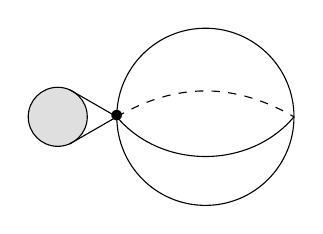
\begin{tikzpicture}[scale=0.75]
      \fill[gray!25] (0,0) circle (0.5);
      \draw (0,0) circle (0.5);
      \draw (2.5,0) circle (1.5);
      \draw (1,0) to[out=-50, in=-130] (4,0);
      \draw (0.2,0.46) -- (1,0);
      \draw (0.2,-0.46) -- (1,0);
      \draw[dashed] (1,0) to[out=30, in=150] (4,0);
      \node () at (1,0) {$ \bullet $};
    \end{tikzpicture}
    \subcaption{$ \tau' $}
  \end{subfigure}
  \caption{Mappe $ \tau_2 $ e $ \tau' $}
\end{figure}
    Poi ho $ \tau' \colon \Disk{2} \to \Sph{2} $ identificazione.
\[
  [\tau'] \in H_2(\Sph{2}) \Rightarrow [\tau'] = \deg{\Delta_\star}[\tau-2]
\]
Cioè
$ \tau_2 \big \lvert_{\partial \Disk{2}} = \tau' \big \lvert_{\partial \Disk{2}} $ sul bordo si
comportano come l'identità, cioè la cella viene mandata in $ \Sph{2} $ meno un
punto. Poi $ A \circ \tau_2 \big \lvert_{\mathrm{int} \Disk{2}} = \tau' \big \lvert_{\mathrm{int} \Disk{2}} $
con $ A $ mappa antipodale, quindi:
\[
  \deg{\Delta_\star} = 1 + (-1)^{2 + 1} = 1 - 1 = 0
\]
Quindi il complesso è:
\[
  \begin{tikzcd}
    0 \rar & \Z \rar{0} & \Z \rar{2} & \Z \rar{0}  & \Z \rar & 0
  \end{tikzcd}
\]
Questo si generalizza immediatamente a $ n $ generico.
Per $ n $ pari:
\[
  \begin{tikzcd}
    0 \rar & \Z \rar{2} & \dots  \rar & \Z \rar & \Z \rar{0} & \Z \rar & 0
  \end{tikzcd}
\]
Per $ n $ dispari:
\[
  \begin{tikzcd}
    0 \rar & \Z \rar{0} & \dots  \rar & \Z \rar & \Z \rar{2} & \Z \rar & 0
  \end{tikzcd}
\]
Si ha l'alternanza di applicazione costante e moltiplicazione per 2.

\section{Successione di Mayer-Vietoris}
\index{Successione di Mayer-Vietoris}

\begin{theorem}
  Sia $ X $ uno spazio topologico e $ A $ e $ B $ sottospazi aperti di $ X $ con la
  topologia indotta, se $ X = A \cup B $ allora esiste la successione esatta di complessi:
  \[
    \begin{tikzcd}
      0 \rar & S_p(A \cap B) \rar & S_p(A) \oplus S_p(B) \rar & S_p(A \cup B) \rar & 0
    \end{tikzcd}
  \]
  Quindi esiste una successione esatta lunga in omologia:
  \[
    \begin{tikzcd}[nodes = {column sep = 10 pt}]
      \dots \rar & H_p(A \cap B) \rar & H_p(A) \oplus H_p(B) \rar & H_p(A \cup B) \rar{\delta} & H_{p-1}(A \cap B) \rar & \dots
    \end{tikzcd}
  \]
  % $ \delta $ è l'omomorfismo di connessione ed è ben definito nel solito modo.
\end{theorem}
\begin{proof}
  Esistono le mappe di inclusione sono $ i_A \colon A \cap B \incl A $ e $ i_B \colon A \cap B \incl B $ quindi
  è ben definita:
  \begin{align*}
    i_\sharp \colon S_p(A \cap B) & \to S_p(A) \oplus S_p(B) \\
    c & \mapsto (i_A^\sharp (c), i_B^\sharp (c))
  \end{align*}
  Ma ci sono anche le inclusioni $ j_A \colon A \incl X $ e $ j_B \colon B \incl X $,
  quindi è ben definita
  \begin{align*}
    j_\sharp \colon  S_p(A) \oplus S_p(B) & \to S_p(A \cup B) = S_p(X) \\
    (a,b) &  \mapsto j_A^\sharp(a) - j_B^\sharp(b)
  \end{align*}
  La successione è esatta, infatti sia $ c \in S_p(A \cap B) $:
  \[
    j_\sharp \circ i_\sharp (c) = (i_A^\sharp (c), i_B^\sharp (c)) = i_A^\sharp (c) -  i_B^\sharp (c) = 0
  \]
  In quanto sugli elementi di $ S_p(A \cap B) $ $ i_A^\sharp $ e $ i_B^\sharp $ agiscono
  allo stesso modo.
\end{proof}

\begin{osservation}
  Questa non è la forma più generale del teorema di Mayer-Vietoris, il quale
  ammette anche la possibilità che $ A $ e $ B $ non siano aperti ma che
  $ X = \mathrm{int} A \cup \mathrm{int} B $, tuttavia questa possibilità si rivela
  necessaria solo in casi patologici.
\end{osservation}

\subsection{Teorema di Jordan generalizzato}

Nel dimostrare il seguente teorema si dà per noto il seguente risultato, la cui
dimostrazione è noiosa e poco istruttiva:
\begin{lemma}
  Se $ f \colon \Disk{r} \to \Sph{n} $ è un embedding allora
  $ \tilde{H}_k(\Sph{n} \setminus f(\Disk{r})) = 0 $, cioè lo spazio
  $ \Sph{n} \setminus f(\Disk{r}) $ è contraibile.
\end{lemma}
\begin{osservation}
  Questo non è un risultato banale perché si dimostra che il complementare in
  $ \Sph{n} $ dell'immagine tramite $ f $ di $ \Disk{r} $ può non essere
  contraibile se $ f $ non è un embedding, come mostrano gli esempi patologici
  del \textbf{Fox-Artin wild arc}\index{Fox-Artin wild arc} o del \textbf{disco
    cornuto di Alexander}\index{Disco cornuto di Alexander}.
\end{osservation}

\begin{theorem}[Teorema di Jordan generalizzato\index{Teorema di Jordan generalizzato}]
  Sia $ f \colon \Sph{r} \to \Sph{n} $ un \textbf{embedding}\index{Embedding}, cioè una funzione
  continua tale che $ f(\Sph{r}) \simeq \Sph{r} $, allora:
  \[
    \tilde{H}_i(\Sph{n} \setminus f(\Sph{r})) \cong
    \begin{cases}
      \Z & \text{se } i = n - r - 1 \\
      0 & \text{se }  i \not = n - r - 1
    \end{cases}
  \]
  Ovvero $ \tilde{H}_i(\Sph{n} \setminus f(\Sph{r})) \cong \tilde{H}_i(\Sph{n - r - 1}) $.
\end{theorem}
\begin{proof}
  La dimostrazione è per induzione su $ r $. Per $ r = 0 $ ho che
  $ \Sph{0} = \set{+1,-1} $, e quindi $ f(\Sph{0}) = \set{p,q} $ essendo un
  embedding. Ho che:
  \[
     \Sph{n} \setminus f(\Sph{0}) = (\Sph{n} \setminus \set{p}) \setminus \set{q} \simeq \RN{n} \setminus \set{\vec{0}} \sim \Sph{n-1}
  \]
  Quindi siccome l'omologia è invariante omotopico:
  \[
    \tilde{H}_i(\Sph{n} \setminus f(\Sph{0})) \cong \tilde{H}_i(\Sph{n - 1})
  \]

  Suppongo di conoscere il risultato per $ r - 1 $: sia
  $ f \colon \Sph{r} \to \Sph{n} $ embedding, considero i due emisferi
  $ \Disk{r}_+ $ e $ \Disk{r}_- $, vale che:
  $ \Disk{r}_+ \, \cup \, \Disk{r}_- = \Sph{r} $ e
  $ \Disk{r}_+ \, \cap \, \Disk{r}_- = \Sph{r-1} $. Sia
  $ U_+ = \Sph{n} \setminus f(\Disk{r}_+) $ e
  $ U_- = \Sph{n} \setminus f(\Disk{r}_-) $, intendo usare Mayer-Vietoris, infatti $ U_- $ e
  $ U_+ $ sono aperti in quanto sono complementari di chiusi in $ \Sph{n} $.
  Ho che:
  \begin{gather*}
    U_+ \cup U_- = \left(\Sph{n} \setminus f(\Disk{r}_+) \right) \cup \left( \Sph{n} \setminus f(\Disk{r}_-) \right) =
    \Sph{n} \setminus (f(\Disk{r}_+) \cap  f(\Disk{r}_-)) = \\
   \overset{\text{$ f $ è embedding}} {=}  \Sph{n} \setminus (f(\Disk{r}_+  \cap  \Disk{r}_-)) = \Sph{n} \setminus f(\Sph{r-1})
  \end{gather*}
  Mentre:
  \begin{gather*}
    U_+ \cap U_- = \left(\Sph{n} \setminus f(\Disk{r}_+) \right) \cap \left(\Sph{n} \setminus f(\Disk{f}_-) \right) =
    \Sph{n} \setminus (f(\Disk{r}_+) \cup  f(\Disk{r}_-)) = \\
    \overset{\text{$ f $ è embedding}} {=}  \Sph{n} \setminus (f(\Disk{r}_+  \cup  \Disk{r}_-)) = \Sph{n} \setminus f(\Sph{r})
  \end{gather*}
  Per Mayers-Vietoris c'è:
  \[
    \begin{tikzcd}[nodes={column sep = 5pt, inner sep = 2pt}]
      \dots \rar & H_{i+1}(U_+) \oplus H_{i+1}(U_-) \rar & H_{i+1}(U_+ \cup U_-) \rar & H_i(U_+ \cap U_-) \rar & H_i (U_+) \oplus H_i(U_-)
      \rar & \dots
    \end{tikzcd}
  \]
  Da cui, utilizzando il precedente lemma ($ H_i(U_\pm) \cong 0 $):
  \[
    \begin{tikzcd}
      0 \rar & H_{i+1}(\Sph{n} - f(\Sph{r-1})) \rar & H_i(\Sph{n} \setminus f(\Sph{r})) \rar & 0
    \end{tikzcd}
  \]
  Da cui passando all'omologia ridotta:
  \[
    \tilde{H}_i(\Sph{n} \setminus f(\Sph{r})) \cong \tilde{H}_{i+1}(\Sph{n} - f(\Sph{r-1})) \cong \tilde{H}_{i+1}(\Sph{n-r}) \cong \tilde{H}_i(\Sph{n-r-1})
  \]
  per ipotesi induttiva.
\end{proof}
\eproof
Questo risultato generalizza il teorema di Jordan\index{Teorema di Jordan} che
dice che se $ C $ è una curva semplice (cioè che non si autointerseca) chiusa in
$ \RN{2} $ allora $ C $ divide $ \RN{2} $ in due componenti connesse.

\begin{example}
  Sia $ f \colon \Sph{1} \to \Sph{2} $ embedding allora:
  \[
    \tilde{H}_i(\Sph{2} \setminus f(\Sph{1})) \cong
    \begin{cases}
      \Z & \text{se } i = 0 \\
      0 & \text{se } i \not = 0
    \end{cases}
  \]
\end{example}

\begin{proposition}
  Il teorema di Jordan generalizzato implica il teorema di Jordan.
\end{proposition}
\begin{proof}
  Sia $ f \colon \Sph{1} \to \Sph{2} $ embedding, $ f(\Sph{1}) $ è una curva chiusa
  semplice, la denoto con $ C = f(\Sph{1})$. Per proiezione stereografica
  $ \Sph{2} \setminus \set{q} \simeq \RN{2} $, dove $ q \not \in C $ definendo
  $ K = \Sph{2} \setminus C $ e $ K' = K - \set{q} $ si ha che
  $ K' \simeq \RN{2} \setminus C $. bisogna mostrare che $ K' $ ha due componenti connesse, e
  questo può essere ottenuto mostrando che
  $ H_0(\RN{2} \setminus \set{q}) = \Z^2 $ e utilizzando il fatto che connessione per
  archi implica connessione.
  % Ho $ \Sph{2} \setminus \set{p} \cong \RN{2} $, per proiezione stereografica, sia
  % $ f \colon \Sph{1} \to \Sph{2} $ embedding, $ f(\Sph{1}) $ è una curva chiusa
  % semplice, la denoto con $ C = f(\Sph{1})$. Mostro che
  % $ H_0(\RN{2} \setminus \set{q}) = \Z^2 $ e quindi
  % $ \RN{2} \setminus \set{q} $ ha due componenti connesse.
  Siccome $ \Sph{2} $ è una varietà topologica esiste un intorno aperto di $ q $,
  denotato $ D $, che è omeomorfo a $ \Disk{2} $, si può sempre scegliere
  questo intorno in modo che non intersechi $ C $. Considerando $ D' $
  intorno aperto di $ q $ si ha che:
  % Poi prendo un intorno $ D' $
  % contenuto in $ D $. Se $ K = \Sph{2} \setminus C $ allora:
  \begin{gather*}
    (K \setminus D') \cup D = K \\
    (K \setminus D') \cap D \sim_H \Sph{1} \; (\text{infatti è una corona circolare})
  \end{gather*}
  % Inoltre $ D \sim_H \set{q} $ quindi $ K \setminus D' \sim K \setminus \set{q} $.
  \begin{figure}[htbp]
    \centering
    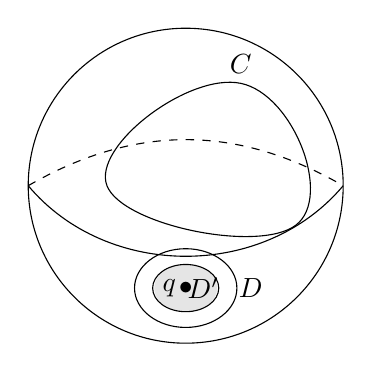
\begin{tikzpicture}
      \draw (0,0) circle (2);
      \draw (-2,0) to[out=-50, in=-130] (2,0);
      \draw[dashed] (-2,0) to[out=30, in=150] (2,0);
      \draw plot [smooth cycle, tension = 1]
      coordinates {(-1,0) (0.7, 1.3) (1.4,-0.5)};
      \node[above] () at (0.7, 1.3) {$ C $};
      \fill[gray!20] (0, -1.3) ellipse (0.4 and 0.3);
      \node () at (0,-1.3) {$ \bullet $};
      \node[left] () at (0,-1.3) {$ q $};
      \draw (0, -1.3) ellipse (0.42 and 0.3);
      \draw (0, -1.3) ellipse (0.65 and 0.5);
      \node[right] () at (0.55, -1.3) {$ D $};
      \node[right] () at (-.1, -1.3) {$ D' $};
    \end{tikzpicture}
    \caption{Teorema di Jordan}
  \end{figure}
  % So che
  % \[
  %   \tilde{H}_i(\Sph{2} \setminus C ) \cong
  %   \begin{cases}
  %     \Z & \text{se } i = 0 \\
  %     0 & \text{se } i \not = 0
  %   \end{cases}
  % \]
  % Ci sono due componenti connesse, infatti per $ i = 0 $ l'omologia è $ \Z^2 $ (infatti
  % l'omologia ridotta toglie uno $ \Z $).
  % % Bisogna dimostrare che $ \tilde{H}_1(\Sph{2} \setminus C) \cong \tilde{H}_1(\RN{2} \setminus C) $.
  % Mostro che $ \tilde{H}_0(\Sph{2} \setminus C) \cong \tilde{H}_0(\RN{2} \setminus C) $.
  % Un modo per farlo è  con Mayers-Vietoris. Sia $ q \in C $,
  % $ \Sph{2} \setminus \set{p} \simeq H_{\RN{2}} \setminus C' $ con $ C' \simeq C $.
  % Voglio mostrare che  $ \tilde{H}_0(\Sph{2} \setminus C) \cong \tilde{H}_0(\RN{2} \setminus C) $
  % implica $ H_0((\Sph{2} \setminus C) \setminus \set{q}) \cong H_0(\RN{2} \setminus C) $.
  % So che per il teorema di Jordan generalizzato $ H_0(\Sph{2} \setminus C) \cong \Z^2 $,
  % devo mostrare che $ H_0(\Sph{2} \setminus C \setminus \set{q}) \cong H_1(\Sph{2} \setminus C) $.
  % Ma questo è ovvio perché togliere un punto non sconnette. In realtà questo non
  % è vero.
  % Voglio mostrare che $ H_q(\Sph{2} \setminus C) \cong H_q((\Sph{2} \setminus C) \setminus \set{q}) $.
  % Prendo $ V(q) $ intorno di $ q $ omeomorfo a $ D $, poi prendo $ D' $
  % e considero $ \Sph{2} \setminus C = K $, quindi $ K \setminus D $.
  % [FIGURA]
  % Uso Mayer-Vietoris $ K = (K \setminus D') \cup D $. So che $ D \sim P $ punto e
  % $ (K \setminus D') \cap D \sim \Sph{1} $ (è una corona circolare).
  Inoltre $ D \sim_H P $, dove $ P $ è l'insieme formato da un solo punto. Quindi
  per Mayers-Vietoris con $ K \setminus D' $ e $ D $ ho la successione esatta lunga:
  \[
    \begin{tikzcd}[nodes={column sep=7pt, inner sep = 1.5pt}]
      \dots \rar & H_1(\Sph{1}) \rar & H_1(K') \oplus H_1(P) \rar & H_1(K) \rar & H_0(\Sph{1}) \rar & H_0(K')
      \oplus H_0(P) \rar & H_0(K) \rar & 0
    \end{tikzcd}
  \]
  So che $ H_1(K) \cong 0 $ per il teorema di Jordan generalizzato e $ H_0(K) \cong \Z^2 $,
  quindi la successione si riduce a:
  \[
    \begin{tikzcd}%[nodes={column sep=3pt, outer sep = 1pt, inner sep = 1pt}]
      0 \rar & H_0(\Sph{1}) \rar & H_0(K') \oplus H_0(P) \rar & H_0(K) \rar & 0
    \end{tikzcd}
  \]
  Cioè:
  \[
    \begin{tikzcd}%[nodes={column sep=3pt, outer sep = 1pt, inner sep = 1pt}]
      0 \rar & \Z \rar & H_0(K') \oplus \Z \rar & \Z^2 \rar & 0
    \end{tikzcd}
  \]
  E quindi $ H_0(K') \cong \Z^2 $.
\end{proof}

\begin{theorem}[Invarianza topologica della dimensione]\index{Invarianza topologica della dimensione}
  Se $ M $ è una varietà topologica di dimensione $ m $ e $ N $ una varietà
  topologica di dimensione $ n $ con $ M \simeq N $ allora $ m = n $, cioè la dimensione
  di una varietà topologica è un invariante topologico: se due spazi topologici sono
  omeomorfi allora hanno la stessa dimensione.
\end{theorem}
\begin{proof}
  Mostro inizialmente che la dimensione di una varietà topologica è legata al
  gruppo di omologia della sfera. Sia $ x \in M $ allora siccome $ M $ è una
  varietà topologica esiste un intorno aperto di $ x $ $ \Disk{m}(x) $, questo
  intorno è omeomorfo al disco aperto $ m $-dimensionale. Sia
  $ U = M \setminus \Disk{m}(x) $, $ U $ è chiuso perché complementare in $ M $ di un
  aperto. Vale che $ \bar{U} = U \subseteq M \setminus \set{x} $ perciò
  $ U \subseteq M \setminus \set{x} \subseteq M $ e quindi posso fare l'escissione:
  \[
    H_i(M, M \setminus \set{x}) \cong H_i(M \setminus U, M \setminus U \setminus \set{x})
  \]
  Ma:
  \[
    M \setminus U  = M \setminus (M \setminus \Disk{m}(x)) = \Disk{m}(x)
  \]
  Quindi:
  \[
    H_i(M, M \setminus \set{x}) \cong H_i(\Disk{m}(x), \Disk{m}(x) \setminus \set{x}) \cong H_i(\Disk{m}, \Disk{m} \setminus \set{\vec{0}})
  \]
  In particolare passando all'omologia ridotta, indicando con $ \Disk{m}_0 =  \Disk{m} \setminus \set{\vec{0}}$:
  \[
    \tilde{H}_i(M, M \setminus \set{x}) \cong  \tilde{H}_i(\Disk{m}, \Disk{m}_0)
  \]
  \begin{figure}[htbp]
    \centering
    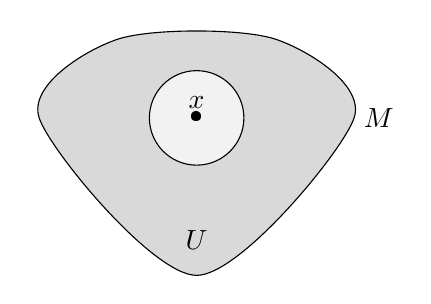
\begin{tikzpicture}
      \fill[gray!30] plot [smooth cycle] coordinates {(0,0) (1,1) (3,1) (4,0) (2,-2)};
      \draw plot [smooth cycle] coordinates {(0,0) (1,1) (3,1) (4,0) (2,-2)};
      \fill[gray!10] (2,0) circle (0.6);
      \node () at (2,0) {\textbullet};
      % \node[right] () at (2.6,0) {$ V $};
      \node[above] () at (2,0) {$ x $};
      \draw (2,0) circle (0.6);
      \node[above] () at (2,-1.8) {$ U $};
      \node[right] () at (4,0) {$ M $};
    \end{tikzpicture}
    \caption{Situazione}
    \label{fig:lez13:dimension_topological_invariance}
  \end{figure}

  L'immersione di $ \Disk{m}_0 $ in $ \Disk{m} $ induce una
  successione esatta lunga in omologia relativa ridotta:
  \[
    \begin{tikzcd}[nodes = {column sep = 7pt}]
      \dots \rar & \tilde{H}_k(\Disk{m}_0) \rar & \tilde{H}_k(\Disk{m}) \rar & \tilde{H}_k(\Disk{m}, \Disk{m}_0) \rar &
      \tilde{H}_{k-1}(\Disk{m} \setminus \set{0}) \rar & \tilde{H}_{k-1}(\Disk{m}) \rar & \dots
    \end{tikzcd}
  \]
  Cioè essendo l'omologia ridotta dei dischi sempre nulla in quanto sono contraibili:
  \[
    \begin{tikzcd}[nodes = {column sep = 10pt}]
      0 \rar & \tilde{H}_k(\Disk{m}, \Disk{m} \setminus \set{0}) \rar &  \tilde{H}_{k-1}(\Disk{m}_0) \rar & 0
    \end{tikzcd}
  \]
  Per cui:
  \[
     \tilde{H}_i(\Disk{m}, \Disk{m}_0) \cong \tilde{H}_{i-1}(\Disk{m}_0)
  \]
  Ma $ \Disk{m}_0 \sim_H \Sph{m-1} $ quindi
  $ \tilde{H}_i(\Disk{m}_0) \cong \tilde{H}_i(\Sph{m-1}) $
  e perciò:
  \[
    \tilde{H}_i(M, M \setminus \set{x}) \cong \tilde{H}_i(\Sph{m-1})
  \]
  A questo punto diventa semplice collegare due varietà differenti: se $ M \simeq N $
  allora:
  \[
    \tilde{H}_i(M, M \setminus \set{x}) \cong \tilde{H}_i(N, N \setminus \set{y})
  \]
  Cioè:
  \[
    \tilde{H}_i(\Sph{m-1}) \cong \tilde{H}_i(\Sph{n-1})
  \]
  Quindi necessariamente $ m = n $.
\end{proof}
\begin{osservation}
  Non vale il viceversa, come ad esempio un toro e una sfera, che hanno la stessa
  dimensione topologica ma non sono omeomorfi.
\end{osservation}

%%% Local Variables:
%%% ispell-local-dictionary: "italiano"
%%% mode: latex
%%% TeX-master: "notes"
%%% End:
